\chapter{Model} \label{chapter-model}
\epigraph{“An economist is someone who says, when an idea works in practice, ‘let’s see if it works in theory.'”
— Walter W. Heller, former chairman of the Council of Economic Advisers.}{ Walter W. Heller, former chairman of the Council of Economic Advisers. (\href{https://quoteinvestigator.com/2015/08/30/practice/}{1979, The Washington Star)}}

\newcommand{\ee}[1]{\color{red}#1 \color{black}}

This chapter links the theoretical discussions of the previous chapters with an agent-based simulation model. The chapter is intended to explain the code and justify the modeling decisions that link the theory to the actual output of the simulations.



\section{The general structure of the model}
Our model has three major components: first, a production function, modeling how urban regions generate wealth,  second a spatial model of an urban housing market, and third, an analysis of distribution within that model that incorporates the financial system.

The social structure of the model begins with  three spatially segregated ``classes.'' Capitalists live in some spaceless utopia, urban workers who commute and earn wages $\omega + w$ in the urban commuter-shed, and  rural landowners who may choose to move to the city. %There may be a band surrounding the city or persons who do not commute but enjoy urban consumption amenities. 

As the model develops, we introduce a land market and allow  the initial urban residents  to retire. They may then  sell or rent out their properties. This introduces a fourth class, the urban tenant. The final agent we add is a bank that represents 
the financial sector, providing mortgage funds and actively purchasing land as a financial asset.



\section{Modelling} 
\subsection{Time}
We imagine the initial set of workers in our city commuting daily, being paid monthly and residing in urban housing for their working lives, which are arbitrarily set. The computational cycle is a year, so all time-dependent variables, such as  wage, transportation cost, and interest rates, are specified for the yearly interval. 



\subsection{Initialization}
Initially, all homes are owner-occupied. This is of interest  as a starting point because we are interested in the evolution of a society with widespread home ownership in the face of financialization pressures. Other initial tenure mixtures are easily modelled.

We also start with owners who have a long run before retirement. The housing market is suppressed during the initialisation runs. The all-ownership, no-turnover case provides a basis for expectation-formation and examining the basic population-productivity dynamic. 


When agents reach the end of their set working lives they retire. It is trivially easy to introduce random life events, but  They may sell their homes and either leave the city or move to cheaper housing.  New entrants to the labour force come from outside of the city at various stages in their life cycle and either buy or rent. homes 



\subsection{Production}
To introduce  the productive nature of cities we  assume the presence of scaling, consistent with neoclassical growth models as discussed in Chapter \ref{chapter-growth}. We treat the estimated scaling relationship as a production function. This allows us to focus on the results of agglomeration in the urban system rather than specifying the system of firms  that transmit the effect. Urban output is more than proportional to urban population: 

 \begin{equation}
 Y\propto N^{\beta} \label{Y}
 \end{equation}

where $\beta >1$.  Equation~\ref{Y} implies , according to neoclassical distribution theory, that the wage premium is increasing in urban  population:

\begin{equation}
\omega\propto N^{\beta-1} \label{MPL}
\end{equation}

Equation~\ref{MPL} says that the city experiences increasing returns to scale in the utilization of human capital. The formulation is  consistent with the discussion of endogenous growth theory in Chapter (Growth), which demonstrated that increasing returns at the macro level is consistent with decreasing returns at the micro level. 

We then treat the city as a single firm facing a fixed price for output. We assume that the firm behaves as a price taker in the labour market as well, despite  the fact that we  model it as a monopsonist.\footnote{Explicitly modelling labour markets with multiple firms is a natural way to specify the model more completely, but it would require introducing many ancillary assumptions and selecting among alternative models of agglomeration, when when we want to focus on distributional and growth-affecting features of the system.}



\subsection{Labour market}
Labour demand is a derived demand based on standard neoclassical theory with an equilibrium wage offer that is the marginal (value) product of labour for the firm. Specifically  hiring proceeds until the marginal product of labour  is equal to the wage.

The firm adjusts its labour force upward when the marginal product of labour is greater than the wage by selecting from its list of job applicants.


The firm adjusts its wage offer upward when the marginal product of labour is greater than the wage \textbf{and} it faces a labour shortage.  Labour shortage is a situation where the firm wants to hire but its list of job applicants is empty.

{\color{red}The details of the adjustment process and the system lags are selected primarily for convenience in simulations. Real-time lags are important and complex, so some sensitivity results will be explored.}

There is no unemployment. there are no labour adjustment costs for firms.



\subsection{Migration equilibrium}
The  productivity of the city attracts people.  In our model, non-urban landowners are those who live too far from the urban job center to justify commuting.  Agents join the urban market by adding their names to the firm's list of job applicants when the rent  on the marginal unit of housing or land exceeds the transportation cost. This is the  standard urban population equilibrium condition. 
   
The growth of population feeds back into productivity. We allow rising population to directly increase the wage.  We model a fairly short lag although in reality lags are long and variable. 



\subsection{Rent}
Rising population and productivity generates an economic value for land that provides proximity to the production center. Use of a unit of land in each cycle is valued at the wage premium net of transportation costs. This quantity is a locational rent. The capitalized value of the locational rent is the property value.\footnote{Note that property taxes reduce the amount of the net locational value that flows to an owner but provides services and wages that make the city attractive. We omit these refinements in this study.}


The rental value of land shapes the city spatially.  We consider a homogeneous city - a single wage, identical preferences, uniform identical transportation costs, identical lot sizes.)



\subsection{The housing market}
Agents enter the urban market two ways. If wages rise, agents just outside the city may become commuters. This increases population. 

When homeowners in the city   retire they sell their home and move to the country. This allows them  to enjoy the capital value of their home.  They either sell their home or rent it to a new occupant. 

When  tenants  in the city  retire they would move to the country to enjoy lower rents. This has no effect on population. It is simplest, therefore to treat tenants as permanent residents unless we want the tenant's  retirement to trigger an event like a rent increase or a decision by the owner to sell the property.



\subsection{Home prices}
The underlying value of a home is the capitalized value of the urban rents, which are perpetual.  Rents, however, depend on urban productivity and may change over time. Any expected increase in future rents should be capitalized into the market price of a home as a capital gain for the owner. Home prices should respond to expectations.

There are reasons to expect the results obtained with  forward-looking agents to differ substantially from those obtained with a model featuring myopic agents.\footnote{For example, Lecca et al. (2013) used a stylized computational macroeconomic model applicable to a regional context to demonstrate that the assumption of myopic vs forward-looking agents yields differences in the dynamics generated by a shock perturbing the initial steady state, even though the alternative paths lead to the same long-run equilibrium.} 

 
\ee{ MOVE TO PRODUCTION CHAPTER?

In this section, we introduce the basic structure of the production side and connect it to the literature on urban scaling. The basic scaling result at the level of the city allows us to incorporate the effect of agglomeration in a standard  circular-city model in a simple way, avoiding the need to explicitly model labour markets and firms.
}



\section{Experiments}
In this section, ] examine the effect of agglomeration, using a circular city model. In subsequent sections we relax assumptions and look at how the interaction between the production of social wealth in cities interacts with housing and the extraction of rent to drive patterns in a richer model with heterogenous agents interacting over space and time. 

% In this section we introduce the production function, introduce the labour supply and the urban model, the source of the surplus,  then we calculate profit, consider who gets the profit, and from there we draw our conclusions.. then we calculate the urban surplus, and consider who gets it. 
%(Derivation details in section \ref{Sec:Derivations})

% \subsection{Labour supply for production}

Following the Alonzo model [], firms are located at the centre of a circular city, the central business district. Residents residents live, spread across the space, and can take jobs and commute to work.
%In the simplest version, firms concentrate at the city centre. Workers are spread over space and pay transportation costs to commute.

Firms produce goods to sell. They can produce more goods by hiring additional workers. 
There is an agglomeration effect, which means firms can also produce more goods by operating in a city with more people, because of the connections and interactions between people (prior section explains and justifies). 
Living close to work has value to workers because it saves the cost of transportation. 

We assume workers receive a subsistence wage, $\psi$, in the countryside, which could come from work in the local community, living off the land, family support, social support, or something else [MAYBE This follows xyz's approach, and makes it possible to explore resident's choice to work]. 

Firms pay a wage premium, $w$, over the subsistence wage to attract workers. 
When workers take a job, they give up the subsistence income and instead receive the wage from their employer. 
The total wage employers pay is thus the subsistence wage plus the urban wage premium  $\psi + w$.

% TODO this shows the dynamics of a local economy, trade dynamics dominate local dynamics in many cases, that is explored with the addition of more cities and centres. 

Workers will go to work if the wage premium is greater than the cost of travel, $\tau$ per unit distance. 
%If the cost of transportation is $\tau$ per unit distance, then t
The farthest workers will travel to work is thus $\frac{w}{\tau}$, which defines the radius of the commuter shed. Thus a worker, located at a distance $d$ from work, paying as much as $w-\tau d$ in rent, would still choose to work, and the distance that workers will commute is limited by to the radius of the commuter shed. Given a standard lot size $s$, the labour available in the circular city is
\begin{equation}L%=  \frac{\pi}{s}(c^{max})^2	
			=\frac{\pi}{s}  \left(\frac{w}{\tau}\right)^2
			=\frac{\pi}{\tau^2 s} w^2, \label{Eqn:LabourSupply1}
	\end{equation}
which increases with the square of the wage.

 % TODO:  FOOTNOTE the transportation cost/distance relationship appears to be non-linear in many cases. While the linear model connects with the established literature, we likely want to explore the implications of more empirically grounded curve (e.g. Alain Bertaud, 2015)



\subsection{Rents}
In the circular city with linear transportation costs, the maximum rent that could be charged for living closer to work is
 \[c^{max}= \frac{w}{\tau}. \]  
 Workers could pay that much in rent and additional costs and it would still worthwhile to commute to work. 

Rents go to the owners of a given property. If workers own their own homes, rents go to them. If others own the land, they can extract the rent. % Rents may also be taxed, could be shared between multiple owners, etc.



\section{Older Drafts?}
Agents purchase homes though a housing market.
In real life, a housing is a market where the product is land with various properties on them. Land value is affected by various elements including proximity to natural features like lakes and mountains, proximity to human-built feature like communities, businesses and amenities, as well a developments and additions on the property itself. 

There is also a layer of policy and rules that determine the land value. For example the city sets zoning rules that allow for certain kinds of uses and disallows others and charges taxes and fees which are factored into the cost structure.

The market is made up of a set of agents who engage directly in the market, including buyers, sellers, renters, investors, developers. 
It also includes others who affect it indirectly including policymakers and those who affect the policy contexts (such as activists, developers, etc), and labour.

%MAIN VERSION HERE IN OVERLEAF UNTIL MOVED BACK

%We build a spatially explicit agent model where agents work in one location and have transportation costs to travel to work. 

This work integrates a model of production and labour into a standard spatial model of the city. 
In this chapter, we introduce an analytic model of production and a labour market in a stylized circular city. 
We develop a spatial model with a labour market and agglomeration effects consistent with the literature as our base model. 
% Extended appropriately, this basic model could be used for planning.
We take a step beyond integrating labour markets in a city, to studying the distributional effects: who gets the surplus, what does that mean for the class structure, and ultimately the productivity of cities? 
% In this section we introduce the production function, introduce the labour supply and the urban model, the source of the surplus, then we calculate profit, consider who gets the profit, and from there we draw our conclusions.. then we calculate the urban surplus, and consider who gets it. 
%In subsequent sections we relax assumptions and look at how the interaction between the production of social wealth in cities interacts with housing and the extraction of rent to drive patterns in a richer model with heterogenous agents interacting over space and time. 
In the next chapter we will integrate a version of this production model in a spatially explicit agent based model with financialized investment. 

This model has three  parts, first a production function, modelling how urban regions generate wealth, and second a model of an urban housing market, and finally, a financial sector that can participate in the market . 
In this section, we introduce the basic structure of the model and examine the effect of agglomeration, using a circular city model.  
\textbf{The model has a Solow-Swan style production model with agglomeration effects using a Cobb-Douglas production function that incorporates Jacobs-style labour-augmenting agglomeration economies %(Beaudry and Schiauerova 2009, Panne 2004, J. Jacobs 1969), 
in the way neoclassical growth theory incorporates labour-augmenting technical change.}
It then integrates the production function with an Alonso-style urban model of a city economy (Alonso 1964). 
It is a model of a productive urban economy since the centre is productive and demands labour.

% Alternative phrasing 
%We integrate a labour market into a spatial urban model, set up to explore rent, and implications for the distribution of wealth.
%This model has two parts, first a production function, modelling how urban regions generate wealth, and second a model of an urban housing market. In this section introduce the labour supply and the urban model, we model the production function, then we calculate profit, consider who gets the profit, and draw conclusions. % The work draws on the Alfonso/Von Thünen model of the concentric city and Dawn Parker and Filatova's work in agent based modelling of housing markets (see http://jasss.soc.surrey.ac.uk/12/1/3.html 2009).% We begin with a simple model of a circular city with urban agglomeration effects. In subsequent sections we will use an agent based model to relax assumptions to look at how the interaction between the production of social wealth in cities interacts with housing and the extraction of rent to drive patterns for individuals over space and time.

The result is a simple model in which marginal productivity determines the wage, the wage determines the size of the city, the size of the city determines the labour supply, and labour supply determines marginal productivity. 
The model is constructed so that there is neither land rent nor capitalist exploitation in the rural economy. 
This special case allows us to examine the distribution of the social surplus generated by agglomeration economies and the effect of financialization.

In the simplest model, the central place pays a uniform wage, $w$ to all employees, who have identical preferences and transportation costs. $w$ is an attribute of individual residents. Residents  purchase or rent equal quantities of land at differing locations $l$ for identical housing.  

There are transportation costs $T$ that depend on distance from the  central place, so land close to the central place is more attractive than land farther from the central place.  

The equilibrium concept is that a market with identical individuals with identical incomes and transportation costs will result in identical utilities. The result is that land rent must decline with distance from the central place to offset rising transportation cost. 

The size of the city is determined by population and lot size. Income and transportation costs will interact with lot size. The basic model can be initialized by matching the number of properties to the size of the population. 



DOES THIS GO TO THE MODEL CHAPTER?

The model is we employ consistent with the theories of Ricardo and Henry George in locating the ground of urban exploitation and class in the capacity to extract social surplus through land ownership, and differs from the standard Marxian analysis in its reliance on access to financial capital rather than control of productive physical capital. The paper concludes that given existing land ownership patterns which encourage speculative investment, housing prices must rise and income inequality must increase. 



We  incorporate Jacobs-style agglomeration economies (\cite{Beaudry:2009ua, Panne:2004vb, JacobsEofC})  similar to the way the  Solo-Swan model incorporates  labour-augmenting technical change using a simple Cobb-Douglas production function.  We bypass the complexity of modelling firms  by allowing population increases  to directly increase urban wage premium.\footnote{The transmission of productivity increases arising from agglomeration effects  to the urban wage through firms, can be modelled in many ways. The agglomeration effects are external to the firm and therefore likely to be unexpected. If  firms underestimate the marginal product of labour, labour productivity will be greater than expected, output will be higher than planned output, and revenue and profits will therefore be higher than expected. Excess demand will attract more productive capital which in turn will demand more labour,  Rising labour demand drives up the wage. The agglomeration effect driving growth is essentially a public good in which individual firms will under-invest. This raises an policy challenge that we leave for others.} %, It is straightforward to compute the rate of excess return for  this model. 
%We insert the production function  into a standard Alonso-style model of a city economy (\cite{Alonso64}). 
In the background, individual firms have decreasing returns, but the presence of agglomeration economies external to firms but internal to the city gives the urban economy as a whole increasing returns to scale. \footnote{These effects can be large. Irwin and Klenow  studied learning in chip production focusing  on the key issue of spillovers. They found learning rates of 10 to 27 per cent, averaging 20 per cent. They indicated that a good part of learning is internal, and that national spillovers were no greater than international spillovers. "... a firm learns three times as much from an additional unit of its own cumulative output as from another firm's cumulative output, regardless of the other firm's country of location. However, rest-of-world cumulative production is typically more than three times any given firm's cumulative production. This means that the absolute contribution of world cumulative production to each firm's experience outweighs the absolute contribution of its own cumulative production. In this sense, spillovers are substantial." (pp. 1217-1218).} 


Rural producers in our model pay a constant wage $\omega$. This is a convenient simplification, not a necessary feature of the model. The urban production sector pays a wage premium $w$.\footnote{
HirschWage (a citation) observe that, ``Following GlaeserMare (a citation),  a  large  empirical  literature  has  investigated differences in wages across labor markets of different sizes. The general finding of this literature is that a significant urban wage premium exists. and that this premium consists both of a level effect and a growth effect that arises as workers gain urban work experience''. } As in the standard circular city model the constraint on growth is provided by transportation costs, which limits the size of the commuter-shed and therefore the labour force at any wage. 



\section{A circular city}

%Call it a radial city?
Following the Alonzo model [], firms are located at the centre of a circular city, the central business district. Residents residents live, spread across the space, and can take jobs and commute to work.
%In the simplest version, firms concentrate at the city centre. Workers are spread over space and pay transportation costs to commute.

Firms produce goods to sell. They can produce more goods by hiring additional workers. 
There is an agglomeration effect, which means firms can also produce more goods by operating in a city with more people, because of the connections and interactions between people (CITE). 
The simple circular city can be extended to to produce other forms, including polycentric cities and hierarchies of cities at the cost of additional computational complexity. The simple case we examine will allows us to focus on the general, and neglected, distributional features of this class of models.

\subsection{Labour supply}

%The wage  determines how far people can travel, since it pays for subsistence, that surplus can go to travel, so the higher the wage, the farther workers travel for work. \note{Maybe } 

Workers in the countryside receive a subsistence wage, $\psi$, which could come from work in the local community, living off the land, family support, social support, or something else. % cite other models with subsistence wage.


% It is convenient in this model to use a Cobb-Douglas utility function that has the property that a fixed fraction of income is spent on housing.  We can start with the assumption that earnings are fixed for the lifetime at the one-period wage, $w$. Then total spending on housing is $\beta Y, \beta <1$ and $ Y=w$. Let the transportation cost for a specific location $l$ be $T(l)$. The  equilibrium price at that location will be $P(l)= \beta Y-T(l)$.


? It is convenient but not necessary to assume that land outside of the residential limit is costless. It is common to assume a fixed price for agricultural land. There is no fixed boundary and the size of the city is determined by the utility that can be achieved in competing regions of competing


Firms pay a wage premium, $w$, over the subsistence wage to attract workers. 
When workers take a job, they give up the subsistence income and instead receive the wage from their employer. 
The total wage employers pay is thus the subsistence wage plus the urban wage premium  $\psi + w$.
Specifying the model in terms of a wage premium simplifies the link to the production side and the treatment of household choice.

The urban wage premium determines how far people can travel. The higher the wage, the farther workers travel for work. 
Workers will go to work if the wage premium is greater than the cost of travel, $\tau$ per unit distance. 
Wage and transportation cost therefor determine the radius of the circular city, which determines the size of the labour force which affects urban productivity.  The cost of travel is therefore an important variable in the development of urban productivity. 

%Living close to work has value to workers because it saves the cost of transportation. 
%We assume workers receive a subsistence wage, $\psi$, in the countryside, which could come from work in the local community, living off the land, family support, social support, or something else. % [MAYBE ADD This follows xyz's approach, and makes it possible to explore resident's choice to work]. 

%If the cost of transportation is $\tau$ per unit distance, then t
The farthest workers will travel to work is thus $\frac{w}{\tau}$, which defines the radius of the commuter shed. Thus a worker, located at a distance $d$ from work, paying as much as $w-\tau d$ in rent, would still choose to work, and the maximum distance that workers will commute is the radius of the commuter shed. Given a uniform lot size $s$, with one worker per unit land, the labour available is the area of the city. In the circular city, this is the area of the circle divided by the lot size
\begin{equation}
                 L%=  \frac{\pi}{s}(c^{max})^2	
			=\frac{\pi}{s}  \left(\frac{w}{\tau}\right)^2
			=\frac{\pi}{\tau^2 s} w^2, \label{Eqn:LabourSupply2}
\end{equation}
which increases with the square of the wage. This is the equilibrium urban labour supply curve.

As in the standard circular city model the constraint on city size and hence growth is provided by transportation costs, which limit the size of the labour force at any wage. 
% Rising transportation costs can become the limit on firm or city expansion. 

%To get wage, we can write thee  inverse labour supply function  is
%\begin{equation}
%	w= (\frac{ \tau^2s}{\pi})^{0.5} L^{0.5},	%\label{Eqn:InverseLabourSupply}
%\end{equation}

 % TODO:  FOOTNOTE the transportation cost/distance relationship appears to be non-linear in many cases. While the linear model connects with the established literature, we likely want to explore the implications of more empirically grounded curve (e.g. Alain Bertaud, 2015)
% More generally, if we were to introduce variations in lot size and housing types  we would want the integral of the worker density function. In our ABM version  of the model we simply count the workers within the commuter shed.

% DETAILS AND ALTERNATIVE PHRASING  
% MARGINAL PRODUCT The marginal product of labour is monotonically declining, ensuring a labour market equilibrium, to connect with the analytic tradition of economic modelling by ensuring there is an equilibrium level of production.  While adding more labour may always adds some value, the rate at which it adds value drops off. 
% If the marginal product increased, then a firm that got large enough would out compete smaller firms, hire all labour, always be able to produce more wealth by hiring more people, and would always produce more wealth by hiring people than by firing people. This doesn't happen. 
% Perhaps, the firm hires employees who best fit its needs first, but to grow, eventually it must hire less selectively. Finding markets may get harder with growth. Perhaps expansion adds additional costs, building a parking lot, administration, acquiring a larger building. Whatever the explanation, the marginal product of labour declines. 

% Frictional unemployment usually just refers to people moving between jobs. When people look for jobs, it may take time to get them. The analytic model offers an equilibrium solution with full employment. In the agent based model this assumption does not hold, workers are laid off, and take time to find new employment.
% labour adjustment costs include moving costs for the employee or hiring, firing, or training cost for the firm. (there might be a hiring, firing, or training cost on the firm side, or on the employee side: expected time to employment costs, moving costs, etc.)
% The assumption of monotonically embedded marginal product of labour is embedded in the production function, so it applies in the analytic and agent models. This appears in the requirement that the sum of the exponents in the Cobb Douglass are less than one without agglomeration effects. Agglomeration effects can push the sum above one. When the exponents add up to less than one, there are diminishing returns to scale.  Exploring alternatives would involved exploring other formulations of the production function.

% $mvp(x) = p(x)$ where x can be labour, capital or any other factor, falls out of the function when you introduce profit maximization. Continuity and differentiability assumed but it is a convenient approximation-- take away assumptions you typically get a close approximation.

%We have a two factor model of production with labour and capital.  







\subsection{Production}

Firms produce goods which they sell in a commodity market\footnote{For simplicity, assume firms produce a variety of perfectly substitutable commodities which are exported and locally consumed at a fixed price in a large market. Note increasing product variety may produce a consumption agglomeration economies as in \cite{FujitaKrugmanVenables}.}. Demand for the urban product is perfectly elastic which means producing more won't affect the product's price; and there are decreasing returns to scale, which means each new worker increases output by less than the last worker did. 
  
We use a two factor model of production, where production, is a function of capital and labour. The firm maximizes profit by setting the marginal value of the product of each factor equal to the unit cost per factor. We model agglomeration with a Solow-Swan style term for labour augmenting technical change. In the Solow-Swan model 

 \begin{equation} 
Y(t)=K(t)^{\alpha }(A(t)L(t))^{\beta }
\label{Eqn:Solow-Swann}
 \end{equation}
where $Y$, $K$ and $L$ are aggregate output, capital, and labour, respectively,  $A$ is the term the Solow-Swan model introduced for technology, that can capture the growth of labour productivity over time, $\alpha$ is the elasticity of output with respect to capital, $\beta$ the elasticity of output with respect to effective labour, and $t$ time. If $\beta=1-\alpha$, this is a constant returns to scale (CRS) production function at the firm level.

% In the Solow-Swan model all factors of production are fully employed, and initial values $A ( 0 )$, $K(0)$, and $n( 0 )$  are given. The number of workers, i.e. labor, as well as the  level of technology grows exogenously at rate %s are $n$ and it   $g$,% respectively:     $L(t)=L(0)e^{nt}$     $A(t)=A(0)e^{gn}$ 
 
This model uses a similar functional form to look at  the effect of population density increasing % productivity. %how density increases in in  % It models how population increases productivity. $\Lambda(n)n$ is  ``effective labor'' 
 the productivity of labour, rather than technology growing productivity over time. With labour augmenting agglomeration, $\Lambda(n)$, in place of technology, the equation becomes 

\begin{equation} 
Y=K_i^{\alpha }(\Lambda(n)n_i)^{\beta }.
\label{Eqn:Prod1}
\end{equation} 
where $n_i$ is the number of workers at the firm, the labour, and $n$ is the urban population. The agglomeration factor increases with population. It multiplies labour because agglomeration scales the productivity of workers. 

A natural functional form of the agglomeration effect for illustrative purposes n is $\Lambda(n) = n^\gamma$. Then:

\begin{eqnarray}
 Y&=K^{\alpha }(n^{\gamma}n)^{\beta}  \nonumber\\
 Y&=K^{\alpha }n^{\beta(1 + \gamma)}.
 \label{Eqn:Prod2}
\end{eqnarray}
If $\gamma=0$ there are not agglomeration effects. Notice that  this formulation implies it is possible to have increasing returns to scale for the urban economy even with a production function at the firm level with decreasing returns to scale: the return to the total economy $\alpha + \beta(1 + \gamma)$ can be greater than one, even if $\alpha +\beta$ is less than one. %.\label{Fn:PSI}}  
(CITE Appendix: Excess Returns)

Assume $\Lambda(1)=1$ so the agglomeration effect has no influence with one person in a multiplicative function like the Cobb-Douglas, and %$\die
FIX die ${\Lambda}{n}>0$, so it is increasing with population.

%%%%%%%%%. ***WHY
If $\beta=1-\alpha$, this is a constant returns to scale (CRS) production function. Without agglomeration effects, $T(n)=1$,  Then  \textbf{$\mathbf{L(n) = T(n) n}$} 

% Without agglomeration effects, $\Lambda(n)=1$,  Then  \textbf{$\mathbf{L(n) = T(n) n}$} }

% Firms will purchase the time of workers to capture the product of their effective labour % and enjoy the product of effective labour. %was If labour markets are competitive, it will set 
%$\die{Y}{L}=w$.
%*** DEFINE EFFECTIVE LABOUR, COMPETITIVE MARKET
% Effective labour is the productive output from labour. As soon as you introduce agglomeration economies, labour becomes a more complex phenomena. There is the benefit of the single worker which should be perfectly declining on that nice concave production function and there is the diagonal movement as a result of increasing productivity because you keep adding people to the market. That means that your productivity of the worker isn't' just attached to the worker and your plant. It has this other component.. 'effective labour' -- the output including the A term.
% Labour always depends on the human capacity, technology, tasks aside so it is always complicated
%Capital is always complicated too it has dates, whether you can get the inputs for it, whether they're produced nearby etc.. -- 

%** ``The notion that your labour force is on average more productive when there are more people around is pretty dramatic and it's very much not part of the basic model that we use. Our starting point is that's the fundamental feature of cities, and what does that do with financial capital and what does that do to distribution and that's not been explored.

%Competitive market- everybody is a price taker they don't assume.
%price takers don't assume anything you do affects other producers or suppliers .. so you act in terms of account your internal prices and costs.
%Take into account any one else's behaviour
%the easy way to see that is assume prices are fixed - all that's required to get the behaviour.

%* have a few other things like free exit and entry, perfect information etc -- to get the efficiency result. - (or to ensure price taking)

%Monopolists knows that increasing output will require a reduction in price-- and take into account how consumers will apply and take it into account.
%No externalities imperfect information etc.. ensure efficiency but aren't needed, all you need is price taking for individuals to only pay attention to their own costs and their own benefits. 

%competitive markets many sellers, many buyers, monopoly single seller, monopsony - single buyer, intermediate cases - monopolistic competition - with some market power but not complete - duopoly- some inefficiency depending on the behavioural model because in the duopoly case they may be able to take advantage of the behaviour of buyers.
% Start with perfect competition, then introduce monopolistic competition is most likely.. but it's more difficult to handle. e.g. with brand names, people have some preference for some feature of your particular good so you can price it higher even though you may loose some marginal people. Firms compete on brand name and reputation, not the pure cost effect.
% In the spatial economy, goods are deferentially interchangeable. Put them on a line and firms pick a place along they line. Firms are in competition but are competing on a line-.. spatial model moved over to characteristic space.. -- looking at this would involve overlaying another space - the characteristic space on the physical space. .. There are also local places with local grocery stores. Polycentric stores have effectively monopolistic competition in real space. - like a named cafe downtown has the same.
% Market power means you can price above marginal costs. Need free entry to get rid of it. -- it doesn't drive out profit - profits can be sustained over longer.
% Monopolist can charge a higher price but pays competitive price for all inputs including labour. If a firm also had a monopoly on offering jobs, they could drive down wages.

%Firms calculate what the next worker is worth to them. That's what they're willing to pay for labour. 
%This is the labour demand function based on the marginal product which is declining. When a firm has only a few workers, it is high on that demand function, and has to move down. It cuts workers. If it's too low, it expands and hires. Note this says something about the geometry of what employers could pay. Firms can't pay workers more than they can earn in the long term, unless that money comes from somewhere, but they could push down wages and extract more profit, invest more in other factors of production, etc

To maximize profit 
% firms set the marginal value product of labour, $p\die{Y_i}{n_i}$, equal to the wage. 
in a competitive market, firms offer a wage equal to marginal value of labour, 
%$p\die
FIX p die ${Y_i}{n_i}$, where $i$ indicates the $i^{th}$ firm. In the analytic model, there is no frictional unemployment, there are no labour adjustment costs.\footnote{Note: we do not assume equilibrium conditions in the agent model, however our approach is to stay close to the analytic tradition, relaxing assumptions to clarify what drives each results, and connect the work with classical and neo-classical theory.}. % For instance in the agent model, employees are simply laid off and seek work, so there is unemployment, but there are not labour adjustment costs for firms.}. For convenience, price per unit is one. 

A labour market equilibrium exists if the marginal product of labour, is monotonically declining, which it is with a Cobb Douglas production function, and $\alpha + \beta<1$ 
Population would be expected to adjust much more slowly than firm wages, so labour supply should converge. The case where there are increasing returns at the city level introduces interesting dynamics, explored in appendix CITE % 'furthur discussion' appendix.

%To ensure there is a labour market equilibrium to study in the analytic model, the marginal product of labour declines monotonically, 
%***ILLUSTRATE AND CLARIFY
%If you see it as just supply and demand .. 
%Supply demand with fixed product and everything’s neat
%Agglomeration changes everything,.. firms are underestimating each time they add a worker, the value that’s going to be produced. They benefit from an agglomeration effect and that’s where they interesting dynamics are coming from..
% we know that there is a marginal product of labour for a firm that it should be able to figure it out.. can the person on the shop floor figure out whether it's worth hiring another person.. we can talk about it, add details etc. We have a declining marginal product of labour. Because of transportation costs, we have a rising cost of getting labour so they cross and there is an equilibrium. There are adjustment questions like which adjusts quickly, how fast people move in, how fast firms decide to hire etc, but we know that there is in principle and equilibrium and that it is in principle a stable equilibrium (DIAGRAM STROGATS) although there are complications with this-- some argue these market equilibria never make sense- true in lots of way, but useful for analysis. 
% The question is then, what happens in our city? Do you get a growth dynamic? What seems to be the case is that if all the firms add workers then the marginal value of the product of all the workers they have goes up, which means they are making more profit which means if they are making more profit they want to hire more workers? Does it ever converge? Likely eventually, but it's got a very powerful dynamic.  If you add other features like more products being created in the city, which is part of this agglomeration process you can start seeing, if you exhaust one source of growth, we know that there are others, that simplification is just firms of the same sort hiring workers of the same sort is wrong. so we need to add the local service sector, we need to add the possibility of creating new products and those depends on the number of workers and so depend on further agglomeration effects. What does this mean? For the purpose of the model, we'd want to strengthen the agglomeration effect relative to what they are for specific firms or industries..

Population/workforce, $n$, and the wage will be determined endogenously in competitive markets. 


 \subsection{Rent}
\label{Sec:Rent}

%``We model how land rent is captured by landowners and how that affects wealth creation and the development of the city. 

%Land is a monopoly good \note{talk about what you mean by monopoly good?} 
The supply of land at any distance from the center is inelastic. 
Its value comes from proximity to the productive urban centre, not from the value of improvements made to the property. 
% Reference sections on development which is different, and the contribution of amenity % Because supply is fixed for urban land, and the landowner has a monopoly claim on rents, the rents that can be depend on wages and amenity rather than the cost of improvements made to the property.
% The source of rents is the free gifts of nature, the coming together of people to create value in cities, and the concentration of public amenity in cities. 
In the circular city with linear transportation costs, the maximum rent for living closer to work is at distance $r$, from the center, is $w-\tau r$.  is Workers could pay that much and it would still be worthwhile to commute to work. 

Rents go to landowners. %the owners of a given property. 
Landowners therefore capture a fraction of the wage premium generated by agglomeration.

If workers own their own homes, rents go to them. If others own the land, they capture them. %\note{REPHRASE? rent is  extracted from the coalition of capital and workers.} % Rents may also be taxed, could be shared between multiple owners, etc. 
%The rents are captured by landowners.  The capture of rents by landowners is common buy not necessary. 
In principle the gains from urban productivity and amenity can be allocated as social wealth through shared ownership, as is often done on a small scale with cooperatives and land trusts, distributed to all citizens through something like a social wealth fund, or captured in taxes or fees as Henry George suggested. 
%The rents would otherwise go to labour and capital.

% Agglomeration benefits get extracted by landowners. Labour gets only their marginal value they don't get any of the surplus. They don't even keep always their marginal value.
the dynamic story is that the class of landowners eventually becomes financial capital.
PLOT RENTS HERE

The value of land increases over time. Those who purchase land earlier claim a share of the growing value of the city. % As the city grows, they own an increasingly valuable asset.
 
%In this model, workers are the initial owners, but they build this wealth which becomes a source of capital that can support them.

EQUATION FOR THE SHARE THEY CAN CAPTURE


\subsection{Demographics}

Workers can leave the workforce and retire, and new people can come into the city. Land value rise as the city grows, so newcomers pay more for housing near the centre.

In the case in which individual workers purchase houses and then sell them on retirement, the housing market drives the creation of classes on its own. A strictly random process in which agents have a range of ages and sell at retirement creates a structural advantage where workers who arrive earlier in the city and own land, benefit from their own labour but also get to claim a share fo the productive output of the city as it grows. % those who begin work later. % to a division in wealth
%the emergence of a class of those who came early and those who came late.
%Early agents may also rent out their land. Could it be though of as a pyramid scheme?

In the classical language, someone is exploited if someone else gets a share of the value of their labour. %(REPLACE WITH MORE PRECISE DESCRIPTION). 
 Employers capture a share of the value of workers' labour, so they exploit workers under this definition.
Those who own land early in a growing city are also capture a share of everybody's production. Since they capture a share of the productivity of others working in the city, through the rents, they are also exploiters, they form a kind of hybrid class. %Rents could be captured directly through renting out the property after they retire away from the city,  or by selling the property at a higher value than they bought it. 

% MARGINALIST DISTRIBUTION
%we've been paying some people less than the market wage so our profits our higher. this is what it would be if we paid everybody
% FOOTNOTE - RELATIONSHIP with marginalist distribution story ******** TODO Does the marginalist approach assume they are not exploited? Is it an experiment in examining the case where production is non-exploitative? 
% In a sense if labour gets the marginal value of their product, are they exploited. It's a matter of interpretation.  -It has an attraction 
%Clark tried to make an ethic of this. if everyone is being paid the marginal product of their labour. We know that's an efficient outcome. If it's efficient, is it also fair
%Is it possible someone's taking out an extra large fair. Yes. Not fair for simple classical reason that labour has been exploited in the past and that the current owner ship is a result of exploitation. The ownership of land introduces a kind of exploitation-- clearly exploitation if you claim that. 
%Lot's of marxists didn't like Henry George making it a locational question, they wanted to keep it located in the factory.
% You could - well what value did they create -- in line with those other-- could interpret.. 
%What is the average value, because every worker is not just marginal, they're also average/identical. What is the value created by the whole of the workforce. Should they be paid the marginal value or the average value of their work.
%
%The avg value -- declining.. 
%The demand for labour is declining--  
%Every infra marginal worker has been paid less than the avg contribution 
%Every infra marginal workers should - 
%every marginal worker should get the average wage.. that's fair.
%
%Get to the margin - that's what you pay.. that's what the next worker is worth to the firm. .. 5th' worker is paid more than the 10th. should it be averaged out and paid to all workers? paid to worker, or should the difference between top and the marginal goes to the firm- -- that's profit.. pay everyone the marginal value and keep the rest as profit.. 
%Effective labour has a higher marginal product.. - even higher - higher for the firm.. - but they don't have to pay the workers that... firms only have to pay enough to get their marginal individual cost down to the wage. The problem there is if they're making more profit they want to expand the workforce, but that wage only supports a certain size of city -- they've got off raise the wage a bit.. so they face an upward sloping supply curve for labour=-- that's why you know there's an equilibrium.. declining product and upward sloping supply so they cross.
%
%(all the profit you earn on the way could be redistributed)



\section{Land Market PROBLEM BELOW}

Urban productivity %and amenity
drives land values through the housing market.%Agents purchase homes to live in. The value of the the proximity to work and to amenity drives shapes the what agents are willing to pay. 
% These prices shape the relationship between housing markets and the wealth of households.
Our goal is to look at the relationship between housing markets, financialized investment, and production. % and labour markets. 
To explore this relationship, we integrate the model of production developed above with a spatially explicit agent based land market. % in which heterogenous individuals and institutions buy and sell properties given their individual goals, resources and available information. We integrate this housing market with % within this model of individual and institutional actors in a spatially explicit property market, a model of production and employment.

We examine the effect of housing on wealth inequality by looking at 
%We explore the wealth forming dynamics of the urban agglomeration effect by modelling 
a city in which agents work in the city and leave their jobs when they reach retirement age. They may choose to rent or sell their home. %?They may chose whether to stay in the city, if there is sufficient amenity value for them, to rent their house, or to sell it. % Todo can agents choose not to retire? Can they keep working? Do they get the subsistence wage on retirement? Do they need to leave the city to get it? 
New agents enter the city to work. 
Agents fund their retirement from savings, as well as returns on their home if they own one. Savings may be invested in a pension fund, or in local property,  depending on expected risks and returns. % either in the stock market, or in pensions.
A financial institution manages the pension, investing in the market or in property.
%Institutional and individual investors can access debt. %We also consider a case where outside money can come under institutional management, not just local retirement savings. A parameter controls the inflow of additional money beyond local investment in the pension fund. 

% There is an outside world in two respects. There is a market for the urban product produced by firms, and a financial market that agents can invest in.
% Lots of simple extensions e.g. 2 cities with immigration, differentiated labour, products, market power, neighbourhood effects (see extensions map/typology), we focus on those elements central to seeing the structure of the resilience dynamics of the wealth/housing effect. Consider adding density, to look at how it interacts with agglomeration effects. (integrating with transportation effects is very neat)
 
 If there is a housing market, agents can move. %In the analytic case above, the population stays in place, and travels to work if it is worthwhile given the transportation costs. 
%Those who come to the city will be those for whom the benefits the city offers make it worthwhile to  whether that's building their network, accessing markets, accessing amenity, learning, finding specialized employment, or increased wages. In this model 
The demand for labour drives urban growth. % The housing market depends on how many people from the periphery are completing to claim places in the city. TODO IF ANY RURAL AGENT COULD MOVE IF THE CITY HAS ADDITIONAL DEMAND FOR LABOUR, HOW DO WE DECIDE WHICH DO? Could use a parameter for immigration (or how 'hot' the market is) and in the simplest case (corresponding to how many agents from outside are looking at the housing/rental market), have the inflow match. % Agents have debt and there is an undifferentiated labour market
 % We may. 
 
Figure xyz traces the flow. In each time step agents firms update wages and job availability, agents decide whether to work and whether to buy and sell homes.
 % Schedule: Multi step by breed
 % Steps Labour
 % step - workers: market/production, enter market to buy, list properties real estate agent matches agents - has bids 
 % bidding - workers and firm consider properties and make bids (2nd step or spread over 2 steps)
 % negotiation - sellers consider and accept bids (or real estate agents manage negotiation)
%Buyers evaluate their need for housing.
% Agents decide whether to enter the housing market as a renter or a buyer.


 
Worker agents from outside the city can always consider moving and accepting a job. % QUESTION - how to manage the flow of new agents?
%, or can make more from rents and moving away (with a non-differentiated workforce)
% They need to approximate housing prices to know if it makes sense to work. Do they use past prices?
% 
% 
The higher their need, the more houses an agent considers, and the more willing they are to negotiate on price. % Buyers rank their housing need on a scale of one to ten. 
% Maybe later: Buyers could consider neighbourhood pressures, demographic changes, changes in job location, desire for amenity etc. in their assessment of housing need. 
Buyers then consult with a financial agent to determine the maximum mortgage and interest rate they'd qualify for based on their income. This gives an upper bound to the range of homes they may consider. 

Next buyers request a selection of homes to consider from a real estate agent. Those with higher need for housing look at more homes. The real estate agent offers a selection of homes based on the agent's requirements. A randomness parameter determines how many divergent houses are also considered. When the parameter is 1, the selection of homes is fully randomized, When it is 0, the agent sorts all available homes and offers those which fit the agents budget, space, and other requirements best.

Finally agents rank all the homes offered and place bids.  For simplicity of implementation, they place bids on all homes they consider. They place the most competitive bids on those homes they prefer. If they have higher urgency they place strong bids on more homes. 
A utility function/algorithm specifies agents preferences over the attributes that matter. - algorithmic continuous. lexographic- any traits. 

Finally Variables from last time also affect desire and urgency in the next time step. If there is a good fit/price ratio, their assessment of desire increases. If they dislike what they see, their desire decreases -- they settle for what is there. 



%Calculate willingness to pay
%Consider options
%Place bids
%
%Calculate willingness to pay (urgency/position on the market)
%Assess need for housing
%- Urgency of need Unhoused, sold house or served notice? 
%- Family or demographic changes
%- Financial viability of current situation
%Assess financial situation
%Get Max mortgage and max carrying cost given income and wealth from a bank
%Get options from real estate agent
%Place bids based on xy
%Consider options
%Place bids
%
%
%
%BUYER
%
%Enter market to buy
%Decide level of urgency (or decide with prospect theory - functional form for optimism/urgency/time to choose)
%(income/wealth)
%Maximum mortgage 
%Maximum carrying cost
%Household attributes - household size, employment location, amenity
%Current housing
%
%Realtor gives list of houses to look (real estate search -e.g. price range)
%Place offers - low if can't afford, higher if market is tight
%If failed, consider renting or buying next time.




\begin{figure}
    \begin{center}
 \tikzstyle{decision} = [diamond, draw, fill=blue!20, 
     text width=4.5em, text badly centered, node distance=3cm, inner sep=0pt]
 \tikzstyle{block} = [rectangle, draw, fill=blue!20, 
     text width=5em, text centered, rounded corners, minimum height=4em]
 \tikzstyle{line} = [draw, -latex']
 \tikzstyle{cloud} = [draw, ellipse,fill=red!20, node distance=3cm,
     minimum height=2em]
%
 \begin{center}
 \begin{tikzpicture}[node distance = 2cm, auto]
     % Place nodes
     \node [block] (need) {Assess need for housing};
     \node [block, below of=need] (finance) {Assess financial situation};
     \node [block, below of=finance] (alternatives) {Select homes to consider};    
     \node [block, below of=alternatives] (bid) {Place bids on homes};    
     % Draw edges
     \path [line] (need) -- (finance);
     \path [line] (finance) -- (alternatives);
     \path [line] (alternatives) -- (bid);        
 \end{tikzpicture}   
 \end{center}
    \caption{}
    \label{fig:code_worker_choice}
    \end{center}
\end{figure}



\section{Financialized capital}

%Individuals and institutions play a role in the housing market through credit markets and direct investment.Agent's access credit shapes worker's ability to purchase homes. Credit is offered by institutions.
% Agents may be able to foresee future growth. %They may even over invest if they follow market trends and bubbles form. 
% They can claim a share of the urban wealth as it grows over time by owning the land. 

If the return on housing investments is competitive with alternative investments, capital from institutions and individuals will flow into housing. Institutional investors can purchase housing.  Individual households can also allocate a larger share to housing to capture the returns.
% If the return on investment in housing is competitive with alternative investments, can purchase housing for it's financial return. They can rent housing and sell the asset with appreciation later. We examine the conditions in which this increased demand can drive up prices in the market. 
% Capturing future growth of the city, depending on their foresight - how much does it take to block individuals from gains-- Regime.
% both institutional investors and individual agents can purchase additional housing for it it's return on investment even though they don't need it as a place to live. 
% Use value vs rent value. 
%Institutional investors can purchase housing as an investment. Individuals with more wealth may invest 
Households may, for example purchase a larger house than they need, purchasing additional units to rent out, or keep a house after retiring rather than downsizing.  % and individuals with sufficient means can purchase larger homes than they need to benefit from appreciation, or purchase additional units to rent to others. 
% Investors can also purchase housing to claim a share of the future productivity of the city. Individuals and groups can put extra money into housing. Institutional housing providers can buy up the housing supply.
% HYPOTHESIS FEEDBACK LOOP -- FINANCIALIZED INVESTMENT --
%The rise in spending on housing as a proportion of income can be driven by both rising prices (cutting into quality of life) and increasing investment to claim a share of the returns.  -- disaggregate and show the geometry -
% Test how linear is this relationship? 

%With financialization, in the case where 
If financialized buyers can access a better interest rate, they can consolidate ownership, capture rents, drive class differentials, and amplify wealth inequality. % This appears to be the case as lenders offer wealthier and larger entities lower interest rates. % We expect to observe in this class of models larger, likely power law-distributed, wealth effects.

%There is a supply of money- if there's too much for other investments, some will flow here- e.g. excess liquidity.



\subsubsection{Size of mortgage available, $m_i$}
\[m_i= \frac{0.25Y_i}{r_i}\]
where $r_i$ is $i$'s cost of capital, $Y_i$ is $i$'s income.

\subsubsection{Cost of capital $r_i$}
The cost of capital is known to differ for rich and poor. Say for example, the cost of borrowing, $r_i$ for agent $i$ if the base lending rate is $\bar{r}$
 \[ r_i = (A + B \frac{\bar{W}}{W_i})\bar r\]
where $\bar{W}$ is mean wealth and $W_i$ is individual wealth. %Figure~\ref{Fig:BorrowingCost} illustrates the effect.

% \begin{figure}[htb]
% \begin{center}
% 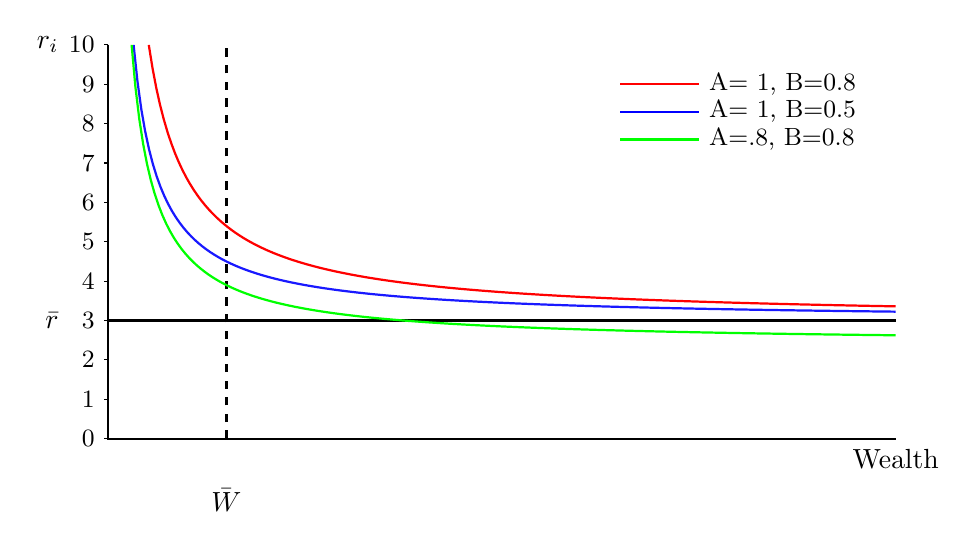
\begin{tikzpicture}[scale=.5]
%\def\bndmax{5}        %https://tex.stackexchange.com/questions/68462/filling-a-complex-region-with-tikz
%\def\bndmin{0.2}
\def \Y {10}  % height of y axis pecent
\def \W {20}  % length  of x axis
\def \Wbar {3} % jmeam wealth
\def \omega {3}
\def \A {1}  %was .5
\def \B {.5}
%Equation   \[ r_i = (A + .5 \frac{\bar{W}}{W_i})\omega\]
\def \Wmin{.63}  %This sets the lower limit fo the 
\def \Wmin{(\B*\Wbar)/(\Y/\omega-\A)} %function to keep in in bounds
	
\tikzset{func/.style={thick,color=blue!90}}	

\draw [thick] (0,\Y)node[left=.5cm]{$r_i$} -- (0,0)--(\W,0)node[below]{Wealth};  	% Axes
\draw [thick] (0,\omega)node[left=.5cm]{$\bar r$} -- (\W,\omega);  	% Axes
\draw [thick,dashed] ( \Wbar,0)node[below=.5cm]{$\bar{W}$} -- (\Wbar,\Y);  	% Axes

\foreach \yi in {0,...,\Y} \draw (0,\yi)--(-.1,\yi)node[left]{\small$\yi$};

\draw[func,domain=\Wmin:\W] plot [samples=200] (\x,{(\A+\B*\Wbar/\x)*\omega});
\def \A {.8}
\draw[func,domain=\Wmin:\W, green] plot [samples=200] (\x,{(\A+\B*\Wbar/\x)*\omega});

\def \A {1}
\def \B {.8}
\draw[func,domain=\Wmin:\W, red] plot [samples=200] (\x,{(\A+\B*\Wbar/\x)*\omega});

\draw [red,  thick](13, 9)--(15,9)node [right, black] {\small A=\ 1,\ B=0.8};
\draw [blue,  thick](13, 8.3)--(15,8.3)node [right, black] {\small A=\ 1,\ B=0.5};
\draw [green, thick](13, 7.6)--(15,7.6)node [right, black] {\small A=.8, B=0.8};
\end{tikzpicture}

% \caption{Hypothetical wealth-dependent borrowing cost}
% \label{Fig:BorrowingCost2}
% \end{center}
% \end{figure}%

This has a number of immediate implications. First, if agents discount at their borrowing rate, wealthier agents a lower discount rate and therefore value properties more highly. 

Second, given the  common rule that mortgage payments cannot exceed some fraction of disposable income, the wealthy will be able borrow larger amounts and at lower interest rates that the less wealthy. At any distance from the centre they will be able to make a higher bid.
 
If the expected return on a property is greater than the individual cost of borrowing, it would pay any agent to borrow as much as possible and purchase properties as they become available.

\subsubsection{The rate of return on a property purchase $v$}
To explore the implication of the financialization of the urban land market we need a function to calculate the return on a unit of land that reflects the actual gradient of opportunity in financial markets. We begin with the price appreciation, $\Delta P=P_T-P_0 = (1+\dot p)P_0-P_0 $, where $\dot p$ is the rate of price appreciation over the period $T$. Rates will all be specified for the period $T$. Transaction costs, including real estate fees, take a fraction from the value of the final sale.

 The speculator invests a down payment, $D$, and gets back at time $T$ the  increased price $(1+\dot p)P_0$, plus rents, minus any costs and minus the mortgage with interest.
%footnote{We can include a use value, $U$ in place of rent for expatriate owners to represent using the property - say one month a year - when they are not renting the property and a \textbf{vacancy tax},
%$T$ at rate $t$ to affect the speculator's  decision.
 
The rate of return is the value of the gain, $V$,  over the size of the downpayment, $D$, where
\begin{equation}https://quoteinvestigator.com/2015/08/30/practice/
V =capital\ gain - Interest\ due  	+ Rent  - operating\ cost\    
\end{equation}

The rate of return is $v = \frac{V}{D}$. 

Both the  share of the price  that can be mortgaged, $m$, and the interest rate  and $r$ may be functions of the agent's wealth. $\delta$ represents the net capital gains tax. It makes it possible to capture the capital gains kept. If it is set to one, it simplifies the equations, all is kept. Keeping the variable offers a policy variable to control the return on financial capital.

\begin{eqnarray*}
V  %	&=& capital\ gain - Interest\ due  	+ Rent  - operating\ cost\\
% 	&=& \delta P_T-D \qquad \qquad \quad - (1+\delta r)M \quad	 + R  	-C\\
% 	&=& \delta P _T \qquad-(P_0-M) \quad- (1+\delta r)M 	 + R  	-C\\
%	&=& \delta (1+\dot p)  P_0 -(P_O -M)  -(1+\delta r)mP_0  + R  -C\\
%	&=& \delta (1+\dot p)  P_0 -P_O + M \qquad -(1+\delta r)mP_0  + R -C\\
%	&=&( \delta (1+\dot p)-1)  P_0  + mP_0 \quad -(1+ \delta r)mP_0  + (\rho-\kappa)P_0\\	
%	&=& \left(  \delta (1+\dot p)-1    + m \quad - m(1+\delta r)  + (\rho-\kappa)\right)P_0\\'
%	&=& \left(  \delta (1+\dot p)-1    + m \quad - m-\delta rm  + (\rho-\kappa)\right)P_0\\
&=& \delta(P_T- (1+r)M) \qquad \qquad 	 + R  	-C   - T\\
&=& \delta((1+\dot p)  P_0- (1+r)mP_0)   + \rho P_0  	-\kappa P_0 - tP_0\\
&=&( \delta((1+\dot p)  - (1+r)m) \ + \rho   	-\kappa -t) P_0
\end{eqnarray*}

This is the  net present value of buying, and selling after one period. \textbf{It has  6 exogenous parameters}. Operating revenue and costs $ \rho -\kappa - t$ a present value. 

The rate of return is $v = \frac{V}{D}$. For expat investors, we get a \textbf{decision rule}:\begin{enumerate}
\item  if $v \geq a$ (with some private use?) with no rent,  don't bother renting. 
\item If $v(no\ rent\ and\ tax) < a\leq v(with\ rent)$,  then  rent. 
\item If $ v(with\ rent) \le a $,  then sell 
\end{enumerate}


We can, with some simplifications, write
\begin{eqnarray}
\frac{V}{D}&=&( \delta((1+\dot p)  - (1+r)m) \ + \rho   	-\kappa - t ) \frac{P_0}{D}   \nonumber\\
		&=&( \delta((1+\dot p)  - (1+r)m) \ + \rho   	-\kappa - t ) \frac{P_0}{P_0-mP_0}   \nonumber\\
		&=&\frac{ \delta(1+\dot p  - (1+r)m) \ + \rho   	-\kappa - t } {1-m} \label{Eqn:DecisionRule}
\end{eqnarray}

\subsubsection{Returns on capital are higher for wealthy investors}

\begin{figure}[htb]
\begin{center}

% Large version
% \begin{tikzpicture}[scale=.5]
% %\def\bndmax{5}        %https://tex.stackexchange.com/questions/68462/filling-a-complex-region-with-tikz
% %\def\bndmin{0.2}
% \def \Y {10}  % height of y axis pecent
% \def \W {20}  % length  of x axis
% \def \Wbar {3} % jmeam wealth
% \def \omega {3}
% \def \A {1}  %was .5
% \def \B {.5}
% %Equation   \[ r_i = (A + .5 \frac{\bar{W}}{W_i})\omega\]
% \def \Wmin{.63}  %This sets the lower limit fo the 
% \def \Wmin{(\B*\Wbar)/(\Y/\omega-\A)} %function to keep in in bounds
	
% \tikzset{func/.style={thick,color=blue!90}}	

% \draw [thick] (0,\Y)node[left=.5cm]{$r_i$} -- (0,0)--(\W,0)node[below]{Wealth};  	% Axes
% \draw [thick] (0,\omega)node[left=.5cm]{$\bar r$} -- (\W,\omega);  	% Axes
% \draw [thick,dashed] ( \Wbar,0)node[below=.5cm]{$\bar{W}$} -- (\Wbar,\Y);  	% Axes

% \foreach \yi in {0,...,\Y} \draw (0,\yi)--(-.1,\yi)node[left]{\small$\yi$};

% \draw[func,domain=\Wmin:\W] plot [samples=200] (\x,{(\A+\B*\Wbar/\x)*\omega});
% \def \A {.8}
% \draw[func,domain=\Wmin:\W, green] plot [samples=200] (\x,{(\A+\B*\Wbar/\x)*\omega});

% \def \A {1}
% \def \B {.8}
% \draw[func,domain=\Wmin:\W, red] plot [samples=200] (\x,{(\A+\B*\Wbar/\x)*\omega});

% \draw [red,  thick](13, 9)--(15,9)node [right, black] {\small A=\ 1,\ B=0.8};
% \draw [blue,  thick](13, 8.3)--(15,8.3)node [right, black] {\small A=\ 1,\ B=0.5};
% \draw [green, thick](13, 7.6)--(15,7.6)node [right, black] {\small A=.8, B=0.8};
% \end{tikzpicture}


\[   r^h=\frac{ \delta(1+\dot p  - (1+r)m) \ + \rho   	-\kappa - t } {1-m}    \]
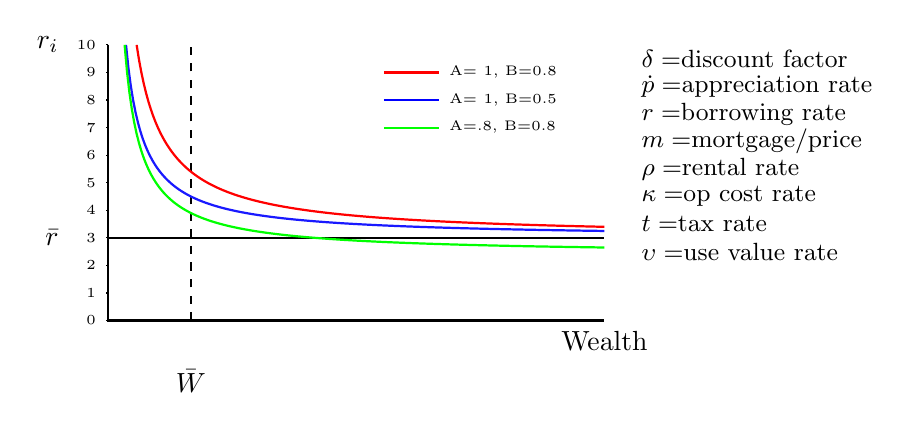
\begin{tikzpicture}[scale=.35]
%\def\bndmax{5}        %https://tex.stackexchange.com/questions/68462/filling-a-complex-region-with-tikz
%\def\bndmin{0.2}
\def \Y {10}  % height of y axis percent
\def \W {18}  % length  of x axis
\def \Wbar {3} % j mean wealth
\def \omega {3}
\def \A {1}  %was .5
\def \B {.5}
%Equation   \[ r_i = (A + .5 \frac{\bar{W}}{W_i})\omega\]
\def \Wmin{.63}  %This sets the lower limit fo the 
\def \Wmin{(\B*\Wbar)/(\Y/\omega-\A)} %function to keep in in bounds
	
\tikzset{func/.style={thick,color=blue!90}}	

\draw [thick] (0,\Y)node[left=.5cm]{$r_i$} -- (0,0)--(\W,0)node[below]{Wealth};  	% Axes
\draw [thick] (0,\omega)node[left=.5cm]{$\bar r$} -- (\W,\omega);  	% Axes
\draw [thick,dashed] ( \Wbar,0)node[below=.5cm]{$\bar{W}$} -- (\Wbar,\Y);  	% Axes

\foreach \yi in {0,...,\Y} \draw (0,\yi)--(-.1,\yi)node[left]{\tiny$\yi$};

\draw[func,domain=\Wmin:\W] plot [samples=200] (\x,{(\A+\B*\Wbar/\x)*\omega});
\def \A {.8}
\draw[func,domain=\Wmin:\W, green] plot [samples=200] (\x,{(\A+\B*\Wbar/\x)*\omega});

\def \A {1}
\def \B {.8}
\draw[func,domain=\Wmin:\W, red] plot [samples=200] (\x,{(\A+\B*\Wbar/\x)*\omega});

\draw [red,  thick](10, 9)--(12,9)node [right, black] {\tiny A=\ 1,\ B=0.8};
\draw [blue,  thick](10, 8)--(12,8)node [right, black] {\tiny A=\ 1,\ B=0.5};
\draw [green, thick](10, 7)--(12,7)node [right, black] {\tiny A=.8, B=0.8};

\def \W {19}  % length  of x axis
\node[right] at (\W,9.5){\small$\delta=$discount factor};
\node[right] at (\W,8.5){\small$\dot p=$appreciation rate};
\node[right] at (\W,7.5){\small$r=$borrowing rate};
\node[right] at (\W,6.5){\small$m=$mortgage/price};
\node[right] at (\W,5.5){\small$\rho=$rental  rate};
\node[right] at (\W,4.5){\small$\kappa=$op cost rate};
\node[right] at (\W,3.5){\small$t=$tax rate};
\node[right] at (\W,2.5){\small$\upsilon=$use value rate};
 \end{tikzpicture}


\caption{Hypothetical wealth-dependent borrowing cost}
\label{Fig:BorrowingCost}
\end{center}
\end{figure}%





\section{Where does this go? Space - describe model logic - VERY OLD DESCRIPTION}


Initialize the model with grid. Each element contains 1 housing unit.

The model space is divided into a uniform grid of single family homes % Additions: apartment buildings, a mechanism to subdivide homes, rent bedrooms, accumulate adjacent land and build new higher density buildings, an urban land boundary, a mechanism for wealth agglomeration through density.

%Household agents have:

\begin{enumerate}
   \item A home. Agents live somewhere, inside or outside the city,
   \item finances: they have assets, a housing budget, income, and a spending pattern - family lending pattern  
   shaped by profession, demographics, family structure, etc.) - risk profile
   \item utility function: they have a utility function with location  preferences    - amenity, open space, house size requirements, transportation costs - shaped by profession, demographics, family structure, etc
\end{enumerate}	

 \subsection{External Capital}
 An investor that buys up assets that cross bellow some lower threshold (threshold is higher during speculative booms), or in consolidating regions.



\section{Savings}
Conventional growth models specify a savings/investment mechanism at the national level. To our knowledge, this has not been done for the city level. We require  savings at two levels. First, since we want to incorporate  households home ownership and a relationship to the financial sector through mortgages, We specify a savings rate out of the spending we have isolated in the `subsistence wage' This means that both urban and rural workers accumulate savings, that savings are age-dependent, making the size of mortgage available also age dependent. 

Homeowners in addition have equity $E=P-M$ in their homes.  ({\color{red}Should newcomers also have equity? or is it built into the savings. Clarify this.} 

A second level of saving is the  investment in capital out of the city surplus. Even raising this question puts us into terra incognita. There are many  channels through which surplus to flows into productive investment in the urban contest. One is through public investment in in infrastructure. We have discussed how falling transportation costs increase surplus generation. Investments like t his are made slowly and take effect over time periods much longer than our model is concerned with.  We can set a property tax rate   that we will assume is sufficient to maintain the stock of infrastructure.

Public and private investment in human capital is largely urban as well, but as with infrastructure, investment and response take effect over time periods much longer than our model is concerned with. 

Private sector innovation in technology, marketing, or products draws on local saving less but still significantly on local savings. We have little in the way of theory or empirical research on this channel. Lags between investment and any rise in the urban wage premium are almost certainly long and variable. 

We deal with this issue by linking local capital ownership with the scale factor. It is known that local ownership is associated with local investment. We will assume that local capital ownership, which consists in part of local ownership of the housing stock, can be proxied by homeowner equity as a share of local. 





\section{The cost of capital}

The cost of capital is known to differ for rich and poor. In our model we  tie the individual cost of capital,  $r_i$ for agent $i$, to a prime rate, $\bar r$ , and to individual wealth. Figure~\ref{Fig:BorrowingCost} illustrates the cost of the borrowing model we implement, 
 \[ r_i = (A + B \frac{\bar{W}}{W_i})\omega\]
Where $\bar{W}$ is mean wealth and $W_i$ is individual wealth. 
\begin{figure}[htbp]
\begin{center}

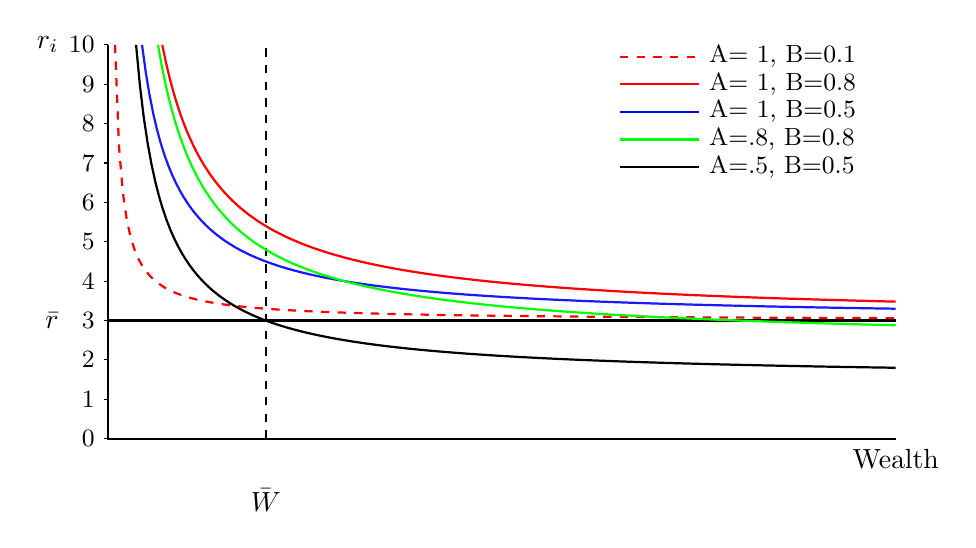
\begin{tikzpicture}[scale=.5]
%\def\bndmax{5}        %https://tex.stackexchange.com/questions/68462/filling-a-complex-region-with-tikz
%\def\bndmin{0.2}
\def \Y {10}  % height of y axis pecent
\def \W {20}  % length  of x axis
\def \Wbar {4} % jmeam wealth
\def \omega {3} % N.B.:  this is r bar

%Equation   \[ r_i = (A + .5 \frac{\bar{W}}{W_i})\omega\]
\def \Wmin{.63}  %This sets the lower limit fo the 
\def \Wmin{(\B*\Wbar)/(\Y/\omega-\A)} %function to keep in in bounds
	
\tikzset{func/.style={thick}}	

\draw [thick] (0,\Y)node[left=.5cm]{$r_i$} -- (0,0)--(\W,0)node[below]{Wealth};  	% Axes
\draw [thick] (0,\omega)node[left=.5cm]{$\bar r$} -- (\W,\omega);  	% Axes
\draw [thick,dashed] ( \Wbar,0)node[below=.5cm]{$\bar{W}$} -- (\Wbar,\Y);  	% Axes

\foreach \yi in {0,...,\Y} \draw (0,\yi)--(-.1,\yi)node[left]{\small$\yi$};

%     ORANGE
% \def \A {1} \def \B {.8}
% \draw[func,domain=\Wmin:\W, orange] plot [samples=200] (\x,{(\A/\x+\B*\X/\Wbar/\x)*\omega});
% \def \A {1} \def \B {.1}
% \draw[func,domain=\Wmin:\W, orange, dashed] plot [samples=200] (\x,{(\A+\B*\X/\Wbar/\x)*\omega});

%     RED
\def \A {1} \def \B {.8}
\draw[func,domain=\Wmin:\W, red] plot [samples=200] (\x,{(\A+\B*\Wbar/\x)*\omega});
\def \A {1} \def \B {.1}
\draw[func,domain=\Wmin:\W, red, dashed] plot [samples=200] (\x,{(\A+\B*\Wbar/\x)*\omega});

%.    BLUE
\def \A {1} \def \B {.5}
\draw[func,domain=\Wmin:\W, blue!90] plot [samples=200] (\x,{(\A+\B*\Wbar/\x)*\omega});
%     GREEN
\def \A {.8} \def \B {.8}
\draw[func,domain=\Wmin:\W, green] plot [samples=200] (\x,{(\A+\B*\Wbar/\x)*\omega});
%.    BLACK
\def \A {.5} \def \B {.5}
\draw[func,domain=\Wmin:\W, black] plot [samples=200] (\x,{(\A+\B*\Wbar/\x)*\omega});


\draw [red,  thick](13, 9)--(15,9)node [right, black] {\small A=\ 1,\ B=0.8};
\draw [red,  thick, dashed](13, 9.7)--(15,9.7)node [right, black] {\small A=\ 1,\ B=0.1};
\draw [blue,  thick](13, 8.3)--(15,8.3)node [right, black] {\small A=\ 1,\ B=0.5};
\draw [green, thick](13, 7.6)--(15,7.6)node [right, black] {\small A=.8, B=0.8};
\draw [black, thick](13, 6.9)--(15,6.9)node [right, black] {\small A=.5, B=0.5};
\end{tikzpicture}


% Figure of cost of borrowing
\caption{Borrowing cost for  $A=1$  $B=0.5$ (blue);  $A=1$  $B=0.8$ (red);  $A=.8$  $B=0.8$ (green);}
\label{Fig:CapitalCost}
\end{center}
\end{figure}
If the expected return on a property is greater than the individual cost of borrowing, it would pay any agent to borrow as much as possible and purchase properties as they can available.\footnote{As pointed out previously,  Equation~\ref{Eqn:DecisionRule} implies a `bang-bang' control - with all sales going to the richest participant unless there are limits on the size of capital flows. For our simulation, we implement such limits. } 
 
The borrowing of most agents will be constrained. A common rule is that mortgage payments cannot exceed some fraction of disposable income. The wealthy will be able borrow larger amounts and at lower interest rates than the less wealthy. 

%The model has been set up so that all of a workers's  income is spent on  basic living costs, $\omega$, transportation $td$ or rent. Disposable income for agent $i$ is therefore just the return  $\omega W_i$ on  financial assets.  

\footnote{Fr\'ed\'erick Demers found that the response of housing investment to interest rates has become more pronounced over time. Modelling and Forecasting Housing Investment: The Case of Canada,  Research Department, Bank of Canada, Ottawa, Ontario, Canada K1A 0G9 fdemers@bankofcanada.ca} 



\section{Model Steps - Housing market}


at every time step 
    1) Some new tenants arrive into the city
    
    2) All unhoused tenants look for a housing unit 
    
        a) They have to decide whether to buy or rent. Decision depends on their income, and the availability of Corporation of Public Housing loans 


        b) If they buy, they seek apartment and evaluate, and place a bid (see ALMA)
        
        c) if they rent, they look for an apartment that matches xyz criteria, and place request to rent. Rental is given by the landlord to the first tenant that matches the asking rental price. 


Workers give up their search and leave the city if they do not find a housing unit 

%\chapter{Background Rought Notes - Rent History Etc}



\section{Agglomeration discussion}

The phenomenon of growing productivity was initially identified and estimated in the economics literature production at the national level. The estimated functions linked capital and labour inputs to output.  Soon after the  earliest econometric models of output  were estimated, it was found that equations were not stable over time. Productivity grew over time
(We can do the arithmetic with the cobb douglas to illustrate) 

Faced with this puzzle, Robert Solow introduced a term that was time dependent, and an entire literature developed to explain this term. One productive stream explained growing productivity in terms of agglomeration effects- more people, more workers more firm or more diversity of firms appeared to be associated with growing productivity. Two major schools emerge - roughly speaking,  the Marshallian explanation, which emphasized firm-level processes and the Jacobs model which focuses on the creative effect of agglomerations of people in cities. Both have receives empirical support.

(We can do the arithmetic with the Cobb Douglas to illustrate)

Louis M. A Bettancourt and others applied similar models at the level of cities, but rather than a time-dependent term, they introduced a population-dependent term and found evidence from cities around the world that productivity rose as population rose: The scale of the city has a positive effect. The result  was one of a wide range of scaling results identifies in a great variety of systems examined in the complexity literature 


\section{Background}

\subsection{Inequality}
this wasn't how capitalism was supposed to work
wages part, 
over 50 for rent

\subsection{Drivers of the housing crisis}
supply and demand, stagnant income, and finacialization of housing

Several explanations of the current situation are commonly proposed. The first is simply that the problem of housing is a supply and demand problem where supply is blocked by some features of urban regulation. The second explanation is that the distribution of income has changed in some way that mean a significant fraction of the population are unable to afford satisfactory housing, and therefore this is the problem that must be solved.  The third common explanation currently is that financialization of the housing market  is changing the way the city economy is working, redistributing income and potentially threatening the long term growth and wealth creating capacity of the city.


\subsection{How we do the resilience analysis}

- what will we do? *** 



\section{Rent, Production and the City: Who Gets the Wealth}


%The sources of economic growth and the distribution of income are themes that run through the history of economic thought. 

The story of rent is the story of 

two great theories of distribution
a methodological evolution from descriiption to calculus to complex systems and an evolution of the economy 
from agriculture to indsutrial produciton, to social scaling or wealht in cities. 



There are two great stories of distribution in economics. The first and oldest is rent, %the classical work on rent, going back to 
developed in Ricardo, in which owners of an asset are able to extract a value beyond what they contribute. 
The second is the marginalist approach, developed by Clark and others, looking at a scenario in which workers receive the marginal value of their contribution to production. This tradition dominate in neo-classical economics, particularly in the United States, and %formed the basis of conventional micro-economics training.
% it gave a story of production that seemed to align with the rising fortunes of ordinary people/workers following WWII, in the 1950s and 1960s when it came to dominate. 
% formed an intelectual foundation for anti-monopoly political movements in the early 20th century. 
This work contributes to a third theory of 

emergent complex systems methodology and  work on urban science, the power law concentration, and integrates/ to achieve a sysnthesis of  the clasical descriptive work on rent and the neoclassical marginalist appraoch

These stories are, at their heart, stories of who claims what share of production. They evolved within an evolving theory of production. The early stories of production thinkers like Ricardo focuses on were agricultural. Who claimed the surplus from agricultural production? Over time, the story moved to industrial production, and increasingly urban- with the social wealth of cities/human capacities developed in cities dominating. % Later thinkers including Smith and Marx%leaving aside purely inherited weath- as that becaumse caught in this same circuit of capital transforming from production, to money and back. 



Methodological-- early discririptive theories told rich layered stories with different
The excitiment concentrated  calculus.. in the classical distributional dynamic.

The complexity - allows for tracing the paths of individual- what happens for whom under a far broader range of conditions

The clarity of pedagogical methcs- bottom up and top up both have illustrative cases e.g. edgeworth box or the schellings/birds models.
But true theory integrates in something that moves between scales fluidly, makes itpossible for the distinct scale based approaches to come together.


Complexity

Early discriptive work
This explosion of formal rigour - focused attention.. 


And the political context..

Monopoly- political pressure real explosion ofwealth creation-- economic success of political efforts to break up monopolies.
And a dynamic- lots of worker power- expanded equality-- workers seemed strong, 
As well as the political environment in the US during the cold war, older stories rooted- marx- repression, ednomists perhaps created an envronment in which economists
a side fo the economcs

-- methological pdrived moved the point whre discriptive and historical appraoches baredly taguth.

Samuelson-- successful exciting-- formal-
a generation
created micro, macro
-- at the moment of the baby boom- departments founded in this moment of exuberance. raised in it, taught according to this framework.


Computers took over from calculus -Brian Arthur
Cities took over from industries - concentrated value-- finance- and law main power centers.. - eigen value centrality.

Crisis in 2008 -- reintroduced dscrptive
Methodologial
Cities-- power law dist. rising debt and inequality. -- unstable and financialize.d
Increasing inequality, risind debt. - worker power expanding wages and equality, a story that explained- vs subsistence.


Exactly what those pattnersnew methods are so succesful are what was lef tout..



Polarized in the periodo of the cold war - the discussion of the market-- perhaps a tendency to avoid the distributionl.. Revolution and drama.



Early theories were implicit. They have the same logic- but exist in words

mathematization was important to the simple centrality of marginalism.






With Clark
A second great theory of distribution
The result is much of the theory of rent was lost. 
time

While Marx emphasized the tendency towards consolidation and exploitation in markets, Clark saw the tendancy to increased competition. 

This allocation— dynamic quality of how wages evolved
They are bidding- and it will converge 
What share do workers get- subsistence wages- get 
But as output grows, and as firms compete for labour, particularly skilled labour, is that a sufficient experience.



Three drivers
Calculus had limits.
The political moment of expanding wages with a labour sector in a position to negotiate as the economy rebuilt following WWII and destruction of old wealth— dynamic time. 
Following WWII with growing demand for labour labour could bargain, 
Following WWII in the period— subsistence waves tending— when labour could bargain,
Following break up some of the largest monopolies like in steak— general steal


Also coincided with the political movement McCarthiesm perhaps led scholars to de-emphasize the connections of their work with the classical socialist litturatue.
Mathematical economics became an exciting and dynamic area.

Until this point the theory was largely descriptive..
xx Cobb working with Douglass developed a formulation — exponential, in economics their names have remained associated with the xyz formulation. 

Clark made a case it was just- became problematic.
Doesn't actually happen -- and not jsut

OUR CASE IS THAT IT FALLS OFF A TOTALY DIFFERENT CLIFF



Economics had theories with rich dynamics, concerned 
Classical economics was concerted with ownership and wealth. But they were largely descriptive.
But the new calculus struggled to deal with stocks and with dynamics. 
(Came back with forester and other systems theory, as well as complexity etc.)

The French Engineers in the school of bridge end road used calculus early .. followed by xyz
Technical development and intelleual excitement aligned
Became very exciting dynamic, had many success - took over the discipline. 
Tied with political successes breaking up big monopolies — seemed to offer a path forward

US opposed soviet ideas and an intellectual environment that may have led academics to dephasize the aspects of their thinking connected with classical socialists thought. 

In this environment a particular approach became dominat— also at a moment when schools and departments were growing— the baby boom came to universities at the moment of Samuelson’s peace micro-macro divide gave a tool kit to a whole generation of economists— 

Embedded at the heart of micro- the satisfyingly precise formal structure of calculus.. the marginalize appraoche— 
Thus came to define a new disciplien— a formalization of Econ.. 
Extensions from that base became the defining advances of a generation of American economists..
Attracted math- a feedback loop.

Less emphasis on intellectual history, how changing- heterodox.. all the full range of thought

Including the much more exiting new techniques of complexity and systems- opening in 2007 an explosion of these techniques in the economies. 




CITIES

But cities matter more and more
Jacobs theory of wealth and value as fundamentally social.. 
Combined with xysz. Jacobs did

Now complexity and scaling theory revealing the universality of those principles advanced by Jacobs..

This requires a different formulation of rent… - and production wealth is inherently social what are the implicaitons— what does that mean.. 






In our model, land comes in implicitly through the demand for labour. 


\section{Chapter: Draft Literature Review and Background}

\section{Background}
\label{Sec:Background}
\newpage
Our approach/model is constructed, drawing together pieces from a number of research areas from economics and the study of cities, including rent theory, production functions, the standard urban model, growth theory, urban growth theories, financialization and the theory of distribution. 
We relate this to the scaling models from the study of complexity. This gives a deeper look at distribution in the cities, the effect of financialization, and effect of both of these on the growth and development of cities. 

The literature makes it clear that the cost of transportation is crucial, the cost of housing is crucial, and that there are strong pervasive agglomeration effects driving productivity and population growth. (City population is observed to follow a power law distribution.)

We are interested in agglomeration economies. The wage  structure would then be related to the population or industry  structure. Externalities driving agglomeration may be classified  into two types, the  or so-called ``Marshalian''  and ``Jacobs'' externalities


3 lines  
- production leading to Jane Jacobs
- cities leading to Jane Jacobs
- scaling factors and complexity leading to Jane Jacobs and empirics in a theory of cities

2 theories of production

Ricardo
Ricardo’s rent theory explained class and the distribution of income in terms of the the productivity and ownership of land in an agricultural society. Land was the scarce factor in production and control of land allowed landowners to extract any production in excess of the agricultural wage. Ricardo could assume that labour was in surplus and therefore the agricultural wage would approximate the subsistence wage. 

Marx
Marx adapted the Ricardian model to an industrial society in which surplus product could be used to create more capital and largely ignored land rents. He retained the subsistence wage, and explored the effect of reproducible capital.

Clark
Clark %\footnote{and Wicksteed} extended the theory of rents to produce 
elaborated a neoclassical distribution theory that tied income to the marginal product of each factor for a firm in a competitive economy rather than class ownership of capital. 
This marginal productivity theory became dominant SOME BENEFITS.. Although the marginal productivity theory became dominant in economic thinking, rent theory retained an important explanatory role in resource, agricultural, regional and later urban economics and even sports economics. 

Clark %\footnote{and Wicksteed} %extended the theory of rents to produce 
elaborated a neoclassical distribution theory that tied income to the marginal product of each factor for a firm in a competitive economy rather than class ownership of capital. Although the marginal productivity theory became dominant in economic thinking, rent theory retained an important explanatory role in resource, agricultural, regional and later urban economics and even sports economics. 

Rent theories have remained at the centre of economics despite the development by Clark (1894) of the more modern theory of distribution in which factors ideally receive the value of their marginal product. In modern welfare economics a measure of surplus that is the direct descendent of Ricardian land rent is at the core of the First Theorem of Welfare Economics, arguably the most significant theorem in the social sciences. With Alonso (1964), another another application of rent theory became the foundation of modern urban economics.

\section{Exploitation}
John Roemer’s 1982 Class Exploitation Correspondence Principle (CECP) states that producers who optimize by only selling labour are exploited at the economy’s equilibrium, and agents who optimize by hiring labour are exploiters. Exploitation and class structure are shown to arise from differential endowments in a manner consistent with both Ricardian explanation of class incomes and Marx’s conception of exploitation. We extend the argument to show that differential access to finance capital, urbanization, the growing importance of human capital in producing surplus and agglomeration economies endogenously generate a class structure based on the indirect capture of land rents, We illustrate the emergence of class structure within a simple agent-based model of the land market in a monocentric city. The model is consistent with the theories of Ricardo and Henry George in locating the ground of exploitation and class in the capacity to extract social surplus through land ownership, and differs from the standard Marxian analysis in its reliance on access to financial capital rather than control of productive physical capital.

The sources of economic growth and the distribution of income are themes that run through the history of economic thought. 

From Smith and Ricardo economist have understood that the net product of the economy is divided among functional classes.
 Ricardo is generally credited with providing the best early description for the division of the product of the land between labour and property owners. 
 Marx is generally credited with providing a convincing explanation based essentially on Ricardo's insights, of the distribution of the product of industrial capital with a class-monopoly on ownership the capital,  as well as insights about the evolution of a society based increasingly on produced rather than natural capital. 
 Henry George elucidated the role of land rent, particularly in the urban context as as a mechanism for extracting socially produced economic surplus.  

The division of the product of the earth among the classes of society has been a central issue in economics since at least Ricardo presented his theory of  rent, through Marx, adapted the concept of rent to an industrial and capitalist economy and Henry George, who applied it in the urban context. Land rent is also at the core of modern urban models.  John %\textcite{RoemerGT} 
in \textit{A General Theory of Exploitation and Class} 

%\textcite{RoemerGT} 
%\footnote{\cite{RoemerGT} p12} 

The distribution of rent, where it goes, and what the implications are. 

\section{Liturature Review}

3 lines  
- production leading to Jane Jacobs
- cities leading to Jane Jacobs
- scaling factors and complexity leading to Jane Jacobs and empirics in a theory of cities

2 distributional stories.
- class and rent -- synthesis of rent and class--

Then is the history of rent seperate?

O’Sullivan (2011) identified “five axioms of urban economics” that have emerged from a century of study: (a) location-specific costs and benefits balance to generate a locational equilibrium; (b) self-reinforcing effects induce concentration of activities and individuals; (c) externalities are prevalent; (d) production is subject to economies of scale, which favours agglomeration; and (e) competition generates zero economic profit. These features combine to produce dynamic urban system that will shape our future. 

We build a model that incorporates the five “axioms” to demonstrate how production externalities, in a class of models, can drive urbanization, class formation and the wealth distribution.

To understand the relationship requires integrating the distributional appraoch from clasical economic theory of rent with the modern marginalist model of distribution through wages. It does this by integrating the urban model with the model of production and including the cost of land and transportation in the urban wage in the labour costs. 
In this way the two factor model of projection reflects the clasical landowning extraction of rents by landowners, with a model of wages in competitive markets. 

\subsection{Rent}

 What Is Economic Rent?






neoclassical story.
Economic rent is an amount of money earned that exceeds that which is economically or socially necessary. This can occur, for example, when a buyer working to attain a good or service that is considered exclusive makes an offer prior to hearing what a seller considers an acceptable price. Market imperfections thus lead to the rise of economic rent; it would not exist if markets were perfect, since competitive pressures would drive down prices. 
%https://www.investopedia.com/terms/e/economicrent.asp
% https://www.wallstreetmojo.com/economic-rent/



Henry George brought the classical position to its logical conclusion: rent is an unearned increment. The Classical Base of Modern Rent Theory, Conway L. Lackman
“Whatever part of the produce or… of its price, is over and above this shame” (which pays for the capital advanced “together with the ordinary profits”), “he” (the landlord) “naturally endeavours to reserve to himself as the rent of his land” ([O.U.P., Vol. I, p. 163; Garnier,]  
l.c., p. 300). Theories of Surplus Value, Marx 1861. [Chapter XIV]  
 Adam Smith’s Theory of Rent [1.  Contradictions in Smith’s Formulation of the Problem of Rent]
This excess may “he considered as the natural rent of land” ([O.U.P., Vol. I, p. 163; Garnier,]
l.c., p. 300).


 \subsection{Ricardo}
 
 David Ricardo developed a theory of land rent.
Leading figure in classical economics



He modelled the agricultural economy.
Ricardo developed the idea of 

He was friends with James Mill, Jeremy Bentham and Thomas Malthus.

He theoriezed the agricultural economy.





\section{Drafting REVIEW}
This section traces the history of rent and production in economics.
 central issue in economics since at least Ricardo presented his theory of  rent, through Marx, adapted the concept of rent to an industrial and capitalist economy and Henry George, who applied it in the urban context. Land rent is also at the core of modern urban models.  


In economics, rent is a surplus value, i.e. the difference between the price at which an output from a resource can be sold and its respective extraction and production costs, including normal return (DFID, 2003; Luchsinger \& M\:uller, 2003; Sharp, 2003; Stoneham et al., 2005).

Chapter 24: Doctrine of Adam Smith concerning the Rent of Land
``Such parts only of the produce of land,” says Adam Smith, ``can commonly be brought to market, of which the ordinary price is sufficient to replace the stock which must be employed in bringing them thither, together with its ordinary profits. If the ordinary price is more than this, the surplus part of it will naturally go to the rent of land.

If it is not more, though the commodity can be brought to market, it can afford no rent to the landlord. Whether the price is, or is not more, depends upon the demand.''

More briefly, rent is a surplus value after all costs and normal returns have been accounted for. Normal costs include  payment of all the factors of production at their market rate.(Labour at the going wage, Capital at the interest rate, supplies at their normal price). The great social question at first was who gets the surplus.  

%The question was pressing because it appeared that landlords were capturing the surplus without contributing to production while may peasants were very poor. 

Ricardo

% Born in the late 1700s, was a British poltical economist. The son of a stockbroker, he built a fortune by investing.
The law of rent was formulated by David Ricardo around 1809, and presented in its most developed form in his magnum opus, On the Principles of Political Economy and Taxation. This is the origin of the term Ricardian rent. Ricardo's formulation of the law was the first clear exposition of the source and magnitude of rent, and is among the most important and firmly established principles of economics.

The landlord would rent out all the land which generated at least enough to pay all the costs. Anything in excess of the costs could be charged as land rent to a tenant farmer.

This excess, or surplus, he identified as the income of the landlord. The landlord captures the surplus by ownership of the natural resource land. 

Ricardo, did not write down a production function his, but his analysis can be understood as implying one.

Clearly in his model there are two basic productive factors, land and labour. The landlord  receives the surplus generated by the land and the rest of the value of production goes to labour. Ricardo essentially assumes that there wage is  just sufficient to reproduce the labouring class.\footnote{``In the natural advance of society, the wages of labour will have a tendency to fall, as far as they are regulated by supply and demand; for the supply of labourers will continue to increase at the same rate, while the demand for them will increase at a slower rate.''  This is  basically Malthus.} He has explained the distribution of the fruits of the land among the main classes of the economy.

The implicit production function is
\[Y=F(N, L)\]

Where the output $Y$ is a function of $N$, the number of workers and $L$, land.

His analysis included a concept of diminishing marginal return, the rate at which production grows declines. 
This shows in his use of the terms ``extensive margin'' and ``intensive margin'' to explain the income of the landowner. He focused on the difference between the cost of production on a unit of land and the revenue generated. 



employers enjoy a bargaining advantage over workers and can coerce them to accept worse terms, because they need individual workers less than individual workers need employment. It is no surprise Marx was an admirer. Wages are not the simple product of supply and demand in Smith; bargaining asymmetries are key.

Ricardo included concept of diminishing marginal product, which means


His analysis can be understood in terms of a production function. 
% Factors of production are things that play a role in creating the output. There are several factors of production, things required for production/to create wealth/value (using capital and labour). Most obviously capital and labour. One of the factors of production is labour. In principle the rate at which hiring changes output can take any form. If hiring one more worker increases output, the marginal product of labour is positive. The marginal product can be positive and increasing, or positive and decreasing. If the marginal product of labour is decreasing, the curve is slopes downward, there are decreasing returns to scale, and each additional worker adds less to output than the last. % DIAGRAM  In general hiring more people increases production. In general employers choose workers who would increase production. Otherwise they would not hire. Returns to scale determins how much hiring one more worker increases output. With increasing returns to scale, each new worker increases output more than the last one did, and companies tend to grow big. With decreasing returns to scale, each new worker increases output by less than the last one did and so more, smaller companies may form % (TODO: clarify explanation of implications). To connect with the tradition of analytic economic modelling, ensure there is an equilibrium, by making the marginal product of labour monotonically declining, ors declining over the whole function. This equilibrium condition ensures the curve in the diagram is slopped downward and the curves intersect. % (TODO: discuss/justify assumption, ground empirically)


 2 factors is typical since it's enough for most kinds of analysis. Another factor typically used to introduce another constraint on production, or potentially consumption. Eg. labour is mobile, capital takes time to accumulate but you can put it anywhere, but forest is a flow from the ground-- puts a limit on the region of the city. - land, flow from the land, natural resources.
 
 The factors are usually chosen so xyz
 To keep it tractable- one which is slow to adjust and one which we can adjust quickly - one which is world/embodied work and one which is current work, the rest falls between.

%and is replaced with capital. -- What you'd do an analysis if you put in 30 factors, in the analysis you hold 28 and let 2 move to see what's going on, and what you get is - you have a production function with certain mathematical factors, you can expand as much as you want. you can expand as much as you like-- everything you deduce about 1 is true about any 1 and all the rest if they hold the same functional relation to one another.This is a mathematical trick that gives you xyz.. things you get from it are things like there's a good reason to assume growth till you get 0 profit, then you get competitive markets, all that drops out of the math. - profit maximization you can impose, expansion to 0 profit, expansion till marginal product of labour equals the wage, value of marginal product of capital equals the interest rate, marginal product of whatever is equal to the price/unit of whatever it is - 


Historic evolution is land and labour.

Marx


, as we move from agriculture, 





John Roemer’s 1982 Class Exploitation Correspondence Principle (CECP) states that producers who optimize by only selling labour are exploited at the economy’s equilibrium, and agents who optimize by hiring labour are exploiters.

Roemer
RoemerGT demonstrates that in equilibrium there are classes that are exploited and classes that are exploiters, as well as intermediate cases, using  a definition a definition of exploitation 

that is essentially Marxian and is consistent with Ricardo's rent theory and that of Henry George: 
%\begin{quotation}
%
An agent is exploited  if and only if the value of the labour the agent sells plus the value of own production plus wage earnings is less than the maximum value of their consumption bundle.
%\vspace{.25cm}
%
%and\vspace{.25cm}
%
%An agent is an exploiter  if and only if the value of the labour the agent sells plus the value of own production is less than the minimum value of their consumption bundle.
%\end{quotation}

A General Theory of Exploitation and Class examined a General equilibrium linear economy in which all individuals rationally choose their  activities given their initial endowments and demonstrated  the endogenous emergence of a class structure in a purely neoclassical model. 

Marx
distribution of the product of industrial capital with a class-monopoly on ownership the capital,  as well as insights about the evolution of a society based increasingly on produced rather than natural capital. 



CITY
Rent howerer has remained central in the study of the city
Began everywhere.

Johann Heinrich von Th\"unen was influential in developing the spatial analysis of rents, which highlighted the importance of centrality and transport. Simply put, it was density of population, increasing the profitability of commerce and providing for the division and specialization of labor, that commanded higher municipal rents. These high rents determined that land in a central city would not be allocated to farming but be allocated instead to more profitable residential or commercial uses. 


 Henry George elucidated the role of land rent, particularly in the urban context as as a mechanism for extracting socially produced economic surplus.  

OLD?
 
Ricardo developed a theory of land rent. He did not write down a production function, but he quite clearly understood and used the concept of diminishing marginal product. This shows in his use fo the terms ``extensive margin'' and ``intensive margin'' to explain the income of the landowner. He focussed on the difference between the cost of production on a unit of land and the revenue generated. The landlord would rent out all the land which generated at least enough to pay all the costs. Anything in excess of the costs could be charged as land rent to a tenant farmer.

This excess, or surplus, he identified as the income of the landlord. The landlord captures the surplus by ownership of the natural resource land. 

Clearly in his model there are two basic productive factors, land and labour. The landlord  receives the surplus generated by the land and the rest of the value of production goes to labour. Ricardo essentially assumes that there wage is  just sufficient to reproduce the labouring class.\footnote{ ``In the natural advance of society, the wages of labour will have a tendency to fall, as far as they are regulated by supply and demand; for the supply of labourers will continue to increase at the same rate, while the demand for them will increase at a slower rate.''  This is  basically Malthus.} He has explained the distribution of the fruits of the land among the main classes of the economy.

The implicit production function is

\[Y=F(N, L)\]

Where $N$ is the number of workerrs

\subsection{Marx}
 Marx examined a developing manufacturing economy. In this economy the owners contributed the machinery, buildings, and even working capita to fund the workers until the product can be sold. This contribution must be accumulated from their profits in the preceding cycle of production,  and has to be reinvested once the revenues of the current round have come in and the bills have been paid. Marx actually describes a circuit of capital from its for as money to its form as physical capital. 
 
 
The implicit production function is

\[Y=F(N, K)\]
where $K$ stands for the productive capital stock. 

As in Ricardo, labour is in surplus and capital is scarce. As in Ricardo the scarce factor owned by a special class - now the capitalists, is able to appropriate the is able to capture the surplus value. Like Ricardo,  marx saw the appropriation of surplus as without morel justification - 


Marx also pointed to a new dynamic in capitalist systems - that productive capital is not fixed as land is, but does and must expand as surplus is reinvested. The expansion will eventually outrun the expansion of demand and the rate of return will fall, leading capitalists unwilling to invest and creating a crisis,.


 
\subsection{Henry George} 
  Henry George returned to land rent with a new insight based on the emergence of the capitalist city. Since land rent is unearned income he argued that it should be seen a social income - that it could be used to pay for all the needs of the community. This is the basis of the `single tax' movement. He cleasrly looks back to Ricardo and the early rent theory, but also forward to urban models. His analysis would be recovered in urban models with the proof of. the `Henry George Theorem" in... by .... It demonstrated that if it was some ;public good that attracted people to a city, the optimal level of the good was jus the amount that could be paid for from the increment in land value.\footnote{Progress and Poverty: An Inquiry into the Cause of Industrial Depressions and of Increase of Want with Increase of Wealth: The Remedy is an 1879 book by social theorist and economist Henry George.}
  
  Wikipedia expresses the dynamics this way: ``The tendency of speculators to increase the price of land faster than wealth can be produced to pay has the result of lowering the amount of wealth left over for labor to claim in wages, and finally leads to the collapse of enterprises at the margin, with a ripple effect that becomes a serious business depression entailing widespread unemployment, foreclosures, etc. ''
  
  In George land includes all natural resources, everything ``that is freely supplied by nature.''  
  \footnote{Analysis of the locational rents generated in this class of models has resulted in several authors demonstrating the validity of variants of the Henry George Theorem (\cite{Arnott-Stiglitz79, Arnott04, BehrensKanemoto14, JohnM.Hartwick1980THGR}). These analyses  show that the land rents can exactly equal the cost of the public good that draws individuals to the city or the production services that draws firms. In our model these rents are extracted by land-owning financial capital. They are not invested in a public good or in expanded production capacity.}
  
  \subsection{John Bates Clark}
  Another socialist like George, he was also one of the pioneers of marginalism. By 1986 he was praising the dynamical process of competition partly in opposition to the single tax movement George had initiated.  His (1891). ``Distribution as Determined by a Law of Rent,'' argued that, given  competition and homogeneous factors of production labor and capital, the division of the social product will be according to the productivity of the last physical input of units of labor and capital.\footnote{Responding to the "indictment that hangs over society" that it involves "exploiting labor," Clark wrote:

    It is the purpose of this work (his 1899 'Distribution of Wealth) to show that the distribution of the income of society is controlled by a natural law, and that this law, if it worked without friction, would give to every agent of production the amount of wealth which that agent creates. However wages may be adjusted by bargains freely made between individual men (i.e., without labor unions and other "market imperfections"0, the rates of pay that result from such transactions tend, it is here claimed, to equal that part of the product of industry which is traceable to the labor itself; and however interest (i.e., profit) may be adjusted by similarly free bargaining, it naturally tends to equal the fractional product that is separately traceable to capital.} 
  
 \subsection{Cobb and Douglas}
 The neoclassical revolution opened the use of formal functional mathematics and calculus. Cobb and Douglas (notably Cobb) came up with a specific and very convenient functional form that captured much of what economists were talking about:
 
 \[Y=AK^\alpha L^\beta\]
 
 Where $A$ is a constant scale factor\footnote {apparently previously used by Knut Wicksell, Philip Wicksteed, and L\'eon Walras. I didn't know that!}. The Cobb–Douglas form was developed and tested against statistical evidence by Charles Cobb and Paul Douglas between 1927–1947. It was  the widely circulated empirical work seems to have permanently associated the rather familiar function with the two names for economists.
 
 A 2021 meta-analysis of 3186 estimates concludes that "the weight of evidence accumulated in the empirical literature emphatically rejects the Cobb-Douglas specification."\footnote{Gechert, Havranek, Irsova, Kolcunova (2021), "Measuring capital-labor substitution: The importance of method choices and publication bias", Review of Economic Dynamics, doi:10.1016/j.red.2021.05.003, S2CID 236400765}
 
 The form captured  important regularities in the data but these drifted over time. 
 
 %COBB DOUGLASS additive property-- multiplicative.. additive property-- expandibile in the sense you can add more in-- some functions which are copb douglas which is log linear so seperable, and so additive in an important sense. BUT MVP is true for any firm successfully multipled function even if pruduction function is not seperable..
 
% Write profit using input, profit, - differentiate, get first order conditions which are a peak in the profit function, take those and manipulate to get rules, features of the optimal behaviour-- set marginal value equal to the price, set quantity to the point where profit goes to zero.. approach to standard economics..
 
 \subsection{Solow}
To deal with the drift, Solow introduced a refinement, opening the field for a further series of refinements  in an enterprise that became known as ``growth theory.'' \footnote{A Contribution to the Theory of Economic Growth,  Robert M. Solow, The Quarterly Journal of Economics, Vol. 70, No. 1 (Feb., 1956), pp. 65-94. Stable URL: http://www.jstor.org/stable/1884513}

Solow argued ``As a result of exogenous population growth the labor force increases at a constant relative rate n,'' so
  \[L(t)= L_0e^{nt}\]


 \[Y=A(t)K^\alpha L^{1-\alpha}\]
 where $A$  explains the change in factor productivity as a function of time. It is no surprise that adding a variable allowed the model to track the data better. Solo went farther and described the dynamics of the model using an explicit time dependence: ``As a result of exogenous population growth the labor force increases at a constant relative rate n,'' so
  \[L(t)= L_0e^{nt}\]
  
  
 As a result, if we stick this into the production function 
 \begin{eqnarray}
 Y&=cK^\alpha (L_0e^{nt})^{1-\alpha}\\
    &=c(e^{nt})^{1-\alpha}K^\alpha L^{1-\alpha}\\
    &=A(t)K^\alpha L^{1-\alpha} \label{Eq:Solow}
 \end{eqnarray}
 where
 \[A(t)=c(e^{nt})^{1-\alpha}\]
 
 N. Gregory Mankiw, David Romer, and David Weil created a human capital augmented version of the Solow–Swan model that can explain the failure of international investment to flow to poor countries.

    \[Y(t)=(A(t)K(t)^\alpha H(t)^\beta L(t))^{1-\alpha -\beta} \]
    
    From the Solow example we can see that if all the time functions are exponential we end up with equation~\ref{Eq:Solow} again.
    
\subsection{How the Solow model performed}    
The estimated model explained 78\% of variation in income across countries, the estimates of $\beta$ implied tha t\textbf{ human capital's external effects on national income are greater than its direct effect on workers' salaries.}%(\url{https://en.wikipedia.org/wiki/Solow\%E2\%80\%93Swan_model)}.  
    
This is interesting for me. I got a similar result. Theodore Breton provided an insight that reconciled the large effect of human capital from schooling in the Mankiw, Romer and Weil model with the smaller effect of schooling on workers' salaries. He demonstrated that the mathematical properties of the model include significant external effects between the factors of production, because human capital and physical capital are multiplicative factors of production.[20] The external effect of human capital on the productivity of physical capital is evident in the marginal product of physical capital:

    \[ MPK={\frac {\partial Y}{\partial K}}=\frac {\alpha A^{1-\alpha }(H/L)^{\beta }}{(K/L)^{1-\alpha} }\]
 
 \subsection{Endogenous growth theories}  
 Endogenous growth theories make the increase in factor productivity depend on an optimizing decisions about human capital investment, invention, investment in technology improvement.  
 
  Productivity growth results from an active search process for innovations in
which the ability to appropriate profits determines the resources devoted to
innovative activity (OECD, 1992, Crafts, 1996). Growth depends on the incentives to in-
vest in improving technology.% https://link.springer.com/chapter/10.1007%2F978-1-349-26732-3_13
 
  I don't think these models are much help in understanding cities, which appear to be come more productive and population rises. this is an agglomeration effect.



\subsection{Solow MORE K}

The firm maximizes profit by setting the marginal value of the product of each factor equal to the unit cost per factor. 

This ensures that the marginal rate of technical transformation equals the price ratio. 

*** WHAT IS THE PRICE RATIO

the marginal rate of technical transformation is the (neg) slope of the indiference curve, 
- technical since it's a technology, the production function representws a technology, and you have inputs-- you can maintain one output by substutiting one input for another, you ocan see them as transfromation (substitution)
- changing technology changes the shape of the curve.. ---note growth theories takes technology out of the term-- growth is a term up front.. on avg it's bringing the whole thing up. consistent with the scaling term-- there is this pre factor that changes a lot- e.g. china to US-- 

NOTE AALSO  the pre factor is by nation not just time-- policy matters weath matters, geopolitical context matters.. a. lot. - US is 8x larger than china 27x larger than nigeria (CHECK NUMBERS..) .. bus driver paid x less.


the indifference curve is the curve along which output stays the same as you supstitute labour for capital or vice versa. 
the optimum input mix, it turns out, is where the isoquant (equal quantity - indifference to quantities curve vs indifference to utilities curve) of the production fuction equals output line is tangent to a cost constraint..

curve tangent to a straight line at the optimum-- at the straight line is the price  ratio

the wage over the interest rate. 

ALTERNATIVE FUNCTIONAL FORMS FOR UTILITY FUNCTIONS AND PRODUCTION FUNCTIONS
isoquant measure how things you eat make you happy-- the production function that has that isoquant is measuring equal outputs
vs indifference curve. .. that has the utility-- is measuring happiness, but they are both the same kind of geometric mean of the inputs. 

Examples whrere the isoquant would not euqal the indifference curve include: -- leiontief for instance- right angle corners with 0 substitution . 2 shoes in a pair. need a left and a right one, two right one doesn't help at all. in that case they're perfect complents not subsitutes
if they're straight line, you have perfect substittes a.. 




\subsection{COBB DOUGLASS PROPERTIES}

We use a Cobb Douglass function for production because it has convenient properties -- you can control the degree of degree to return to scale simply by varying alpha and beta. secondly alpha turns out to be under the marginal productivity interpretation of income and optomixation, it ends up being the share of income that goes to capital and to labour- ends up being the elasticity of capital with respect to labour or elasticity of capital with respect to labour.. very much a funcitonal form in line with the scaling  appraoch and they come to the same.. -let's you talk about your returns to scale naturally and ascribe them as you will. it also -- really convenient form used throughout econ for illustration, it has been estimated, and it can be derived alternatively as the form you can look for from the scaling research..]
*** XYZ properties,

cobb douglass has another trait, which is it's a constant elasticity of substitution fuction.
elasticity of subsstittuion combines the slope and the amt of inputs. . easy to slow graphically CEF - constant elasticity of substitution.




Growth theories have several components
the amt of each you have

e.g. if an economy increases the labour or capital it has, it can move to a higher isoquant. if it increases 1 it can move to a higher isoquant-- that doesn't change the shape-- you can move since you have more inputs.

if you have technical change that makes 1 factor more productive.. imagine a nice smooth isoquant.. and it takes some labour that puts you on that isoquant.. if the labour got more producteive, the same amt of labour would move you to a higher isoquant.. cou..


Solow swan puts tech to the front-- the prefactor containts tech growth

we actually put the factor of production into the prefactor.. ** 



% Note on functional form: The analytical approach looks at marginal product and curvature of these functions -- so all we need is something with a curvature and a marginal product in each factor that you put in -time capital, labour 1, labour 2, labour 3.. our focus is on the local curvature and the slope.
%(\cite{Solow56, Swan}), 


VARIATIONS

There are all kinds of other things that could be included in Solow-Swann. For instance, the Mankiw–Romer–Weil version of the model adds a term for human capital.

The general form can be extended in many ways 0 
 In principle it could be restrictred offer time, different workers, firms, sectors, neighbourhooods, evolving over time.


\subsection{Exploitation}\label{Sec:Exploitation: A Note}
The division of the product of the earth among the classes of society has been a central issue in economics since at least Ricardo presented his theory of  rent, through Marx, adapted the concept of rent to an industrial and capitalist economy and Henry George, who applied it in the urban context. Land rent is also at the core of modern urban models. 
%John \textcite{RoemerGT} in \textit{A General Theory of Exploitation and Class} examined a General equilibrium linear economy in which all individuals rationally choose their  activities given their initial endowments and demonstrated  the endogenous emergence of a class structure in a purely neoclassical model. 

%\textcite{RoemerGT} demonstrates that in equilibrium there are classes that are exploited and classes that are exploiters, as well as intermediate cases, using  a definition a definition of exploitation\footnote{\cite{RoemerGT} p12} that is essentially Marxian and is consistent with Ricardo's rent theory and that of Henry George: 
\begin{quotation}

An agent is exploited  if and only if the value of the labour the agent sells plus the value of own production plus wage earnings is less than the maximum value of their consumption bundle.\vspace{.25cm}

and\vspace{.25cm}

An agent is an exploiter  if and only if the value of the labour the agent sells plus the value of own production is less than the minimum value of their consumption bundle.
\end{quotation}

Class position is shown to depend on initial endowments. 
Our model also reveals classes that capture surplus generated by the labour of others. In our model the process is driven by agglomeration economies and urbanization. The analysis does not depend on whether we accept the notion of exploitation presented by Roemer, Marx or any other theorist. We simply note that the model generates classes in a well defined sense, and a division of that surplus among those classes that can be understood  as exploitative in the  classical sense. 







\subsection{Facts justifying our model}

The New Geography of Jobs - what's scarce is tallent. There is catastrophic agglomeration and a growing divide
and those in the good parts cant even afford to own that future, and those outside have no claim even on the income, joy or the chance at a family it offers.

It is debt farmed for ideas till it sheds its' need of you. 
The. actuall needs of humans could sputter out. but what is happening now is simply the draining

the continued logic of extraction.
Tbe logic- it can go somewhere else so ti flows around till place is destroyed. 

the other logic is investment. it looks amost the same. still uses prices, choices, the adjustment so it has alittle more humanity than the naked logic of the individual. -- still spend alone or together. still tu

but the more that stays local the better. and a certain amount stll builds up== the principle builds- the human expression of capacity--

-** all value is craeted for itself. except alienated value. Marx believed the alienation was endemic, but there's a more basic shift in what is needed-- we are needed, at least a few of us as full humans.

--- it is unpredictable

Winner take all-- means everyone gets the best thing. 

The problem of distribution has become the big thing
wealth is connection-- it is the productivity of the dense clusters.. 
Every urban boundary iatrs a potential. we could simply cross the line and install a new logic

1. you'd need a mechanism to drive density- to fight nimbyissm -- the inexorable drive of the markt to unlock an unwillign strivign 
and 
2. you'd need

can we choose a better world ourselves or must we be trappe din it.

of course allow as many other worlds to flourish. most of the world will be free for other worlds so that is no problem.. not even a contracdiction. a new wildness will be on offer, an enw pastoralsim an solw travel airships. 

I have dreamed a few times and cast my webs. played in the eddies of the dancing shimering world as it comes into being. I was at blackberry when it was everywehre, walked in the washinton where it was thew first thing each reached for in the morning and dreamed of the clean lines of the screen ot the edge, the ocmputer. and then held that very thing I'd dreamed of in my hands,

the edge of the inexorable world. anyone can go there and dream and some rutheless one can claim a little share of it.
most will be harvested by the little spiede3rs from law school hwo sit in the corners and and pounce with words never met from it
reality- they are the matrix keepers-- they keep oru constraints in place, they ony thing that takes out enough of our free choice that wecan be predicted and better managed a little

-- it is only the unexpected that is not claimed.
the ghosts of bubbles past.
the hangofers
the feelings never felt

if death iddn't exist we'd invent it
if place didn't exist we'd invent it

we just wiped out something we now have to cojure up but it is just place. a simple thintg not like the dead dancing spiders who well never come back on the odle ear= who will never danc again.
not like the spiders who will never dance in their colours again

come to the museum and see it
be hungry for the flavors adn spices of the world-- see the world -- meet people all over the world killthem.
what can you see, what can you take.

the flowering of the colision
and how few survive it.

but we in the wake of that exploseion. the attom unlocked bust now invent place.

cities were privates.

they are only freed for a moment when they realize that the free mind creates. but it is in a box.

free us all and you can only imagine what we'd make

the pale impovrished publics. the mall is is just a mockery of the public world-- fo the genuine quality of the backyard gathering. 

'Global inequality is not natural, inevitable, or accidental' Jason Hickel The Divide: Global Inequality from Conquest to Free Markets - give aid, they'll get institutions and get rich, but it's a lie of course.
The division is structural.

Have your diversity clubs, but they still cut to the bone, and drive you till your dead. You already adopt an alienated language- runing things up the flag pose. Cliches you'd never dream of in scohol. And so it is just one more thing to control your eyes when the races flash before you on the 'race' tests, just one more false alienated language to adopt. 
And it is all helpsless when it -
and you run farther and farther and still own nothing. Just another day older anddeeper in deblt
But we've sung labour songs for generations. And what we sang is in our bones, it will take more than these false words to cut it off of us. 
I don't want words they say.
I want a way out. I want hope. But even hope smarts, too fresh a promise broken. I cannot vote for hope again, though I cry every time it wins. Another neo-liberal lie

liberalism is this grand dream of liberty and hope. 
But if you don't have the guts
the only dream that cant be co-opted is one that wins.
And it never even tried to win. It never even cared. 


So yes dream of liberty. Drean of truth, and the skyline of forever. But don't dry to me if walking on dreams takes you no-where real.
but don't hit the dreamers.
Hit the liars and the theifs who never gave it a chance.
The ideal was so magical-- so dense, that the worst among it hid in its vabours. 

so densse, lofty diaphanous. Who tood up it's words.
Words. Words. 
The wordy will take them first.

The anti-racist neoliberal beast.
The xx family was the only one to ever embrase the entreprenru.

Great ideas have been peformed. 
And who knows if that's all constatintoble did when he saw the x in the sky and united gentile and jew in the greatest army him history, and binding our god in the. 
But she's free now. The Volcano brought her out. 
And so maybe god is dead. I tried to read him and could get nothing but an empty space.
IT took some time. 
But it is easiery to predict history
But it is easier to predict the future than to say when it will happen

Maybe we can wipe clean our failures now. 
Maybe that slow adoption is ready to speed up.

An emergency is not done by giving up before our time has come. 
Can you make this an experience. 




\subsection{There is an urban rent premium/scaling effect}
There is an urban wage premium %\textcite{HirschJahn} observe that, ``Following \textcite{GlaeserMare}   a  large  empirical  literature  has  investigated differences in wages across labor markets of different sizes. The general finding of this literature is that a significant urban wage premium exists. and that this premium consists both of a level effect and a growth effect that arises as workers gain urban work experience''.

applies most in tech economies like waterloo (maybe also with univerity,   info econ)

applies most with strong urban boundary -- functions essentially as a potential-- could grow with density- urban grows s ti grow the potentieal as well s the wealt-- adds a resilience benefit-- that's why exploiters sees to suc out

scaling laws- socioeconomic outputs scale for the reasons we say.


\subsection{Henry George Results}
Analysis of the locational rents generated in this class of models has resulted in several authors demonstrating the validity of variants of the Henry George Theorem (\cite{Arnott-Stiglitz79, Arnott04, BehrensKanemoto14, JohnM.Hartwick1980THGR}). These analyses  show that the land rents can exactly equal the cost of the public good that draws individuals to the city or the production services that draws firms. In our model these rents are extracted by land-owning financial capital. They are not invested in a public good or in expanded production capacity.

\subsection{Modelling Notes}


simple model justified when there are unknowns % - consider largest uncertainty not just largest data volume - highly available data in part of a model can tempt to complicate a model.. model simplicity should be constriande by the least of data rather than the most. . tend to use all the data we have can unballance

\subsection{How our model compares with other models}

- an origin story, and a test bed-- a grounding that ties it rigorously with the neoclassical model-- 


contrib - a novel intervention, based on a novel theory, recognizing an unusual opportunity- within this region.

contrib - It appears that the analysis of  agglomeration effects has not explored what the endogenous growth literature has to offer.

Production is by firms at the center. The production economy is what generates a surplus.  % This means we have a production/production economy. %, while many models of wealth distibution look at capital and financial markets, 
- vs lots of econo physics models looking at trades/markets rather than production.

Land plays a role in production, but not as a formal factor in the production function, but turns out to be a limit on output. The transportation cost ties labour to land. 

With agglomeration, firms produce more by being near more people.

We put the agglomeration factor in the bracket with labour because agglomeration scales the produtivity of workers.
we actually put the factor of production into the prefactor

The scale litturature comes to the same model with a different derivation, the relationship is traced in Section \ref{Sec:Scale} on Scale. 

 CUT? This differs from  the Slow-Swan, model in which labour augmenting technical change increases according to an exogenous (exponential) - but it's equivalent to the scaling law.

Notice that this model ascribes the agglomeration effects to labour rather than capital. Deepening  and widening of the labour pool was one of Marshall's explanations of the formation of industrial districts. 
The model can therefor  be seen as incorporating a Jacobs/Marshall externality (\cite{Beaudry:2009ua, Panne:2004vb}) of the sort often invoked as an explanation of industrial clusters. 
These externalities  are not a product of any firm or individual, they come from the social interaction of many people.

\subsection{Pictures of the model}

% In Figure~\ref{Fig:Rent1} 
the blue line is a conventional urban rent profile. $A(0)$ represents the effect of including a consumption externality as we do later.  For  $A(0)=0$ the orange line and orange block disappear. 
The social surplus generated by agglomeration effects in production appear as the white triangle below the blue line. The social surplus generated by agglomeration effects in consumption appear as the difference between the blue line and the orange one.
%\begin{figure}[htbp]
%\begin{center}
%\input{SA_RentProfileClasses.tex}
%\caption{Rent profile and population segregation with amenities}
%\label{Fig:Rent1}
%\end{center}
%\end{figure}



